% Options for packages loaded elsewhere
\PassOptionsToPackage{unicode}{hyperref}
\PassOptionsToPackage{hyphens}{url}
%
\documentclass[
]{article}
\usepackage{amsmath,amssymb}
\usepackage{lmodern}
\usepackage{iftex}
\ifPDFTeX
  \usepackage[T1]{fontenc}
  \usepackage[utf8]{inputenc}
  \usepackage{textcomp} % provide euro and other symbols
\else % if luatex or xetex
  \usepackage{unicode-math}
  \defaultfontfeatures{Scale=MatchLowercase}
  \defaultfontfeatures[\rmfamily]{Ligatures=TeX,Scale=1}
\fi
% Use upquote if available, for straight quotes in verbatim environments
\IfFileExists{upquote.sty}{\usepackage{upquote}}{}
\IfFileExists{microtype.sty}{% use microtype if available
  \usepackage[]{microtype}
  \UseMicrotypeSet[protrusion]{basicmath} % disable protrusion for tt fonts
}{}
\makeatletter
\@ifundefined{KOMAClassName}{% if non-KOMA class
  \IfFileExists{parskip.sty}{%
    \usepackage{parskip}
  }{% else
    \setlength{\parindent}{0pt}
    \setlength{\parskip}{6pt plus 2pt minus 1pt}}
}{% if KOMA class
  \KOMAoptions{parskip=half}}
\makeatother
\usepackage{xcolor}
\IfFileExists{xurl.sty}{\usepackage{xurl}}{} % add URL line breaks if available
\IfFileExists{bookmark.sty}{\usepackage{bookmark}}{\usepackage{hyperref}}
\hypersetup{
  hidelinks,
  pdfcreator={LaTeX via pandoc}}
\urlstyle{same} % disable monospaced font for URLs
\usepackage[margin=1in]{geometry}
\usepackage{graphicx}
\makeatletter
\def\maxwidth{\ifdim\Gin@nat@width>\linewidth\linewidth\else\Gin@nat@width\fi}
\def\maxheight{\ifdim\Gin@nat@height>\textheight\textheight\else\Gin@nat@height\fi}
\makeatother
% Scale images if necessary, so that they will not overflow the page
% margins by default, and it is still possible to overwrite the defaults
% using explicit options in \includegraphics[width, height, ...]{}
\setkeys{Gin}{width=\maxwidth,height=\maxheight,keepaspectratio}
% Set default figure placement to htbp
\makeatletter
\def\fps@figure{htbp}
\makeatother
\setlength{\emergencystretch}{3em} % prevent overfull lines
\providecommand{\tightlist}{%
  \setlength{\itemsep}{0pt}\setlength{\parskip}{0pt}}
\setcounter{secnumdepth}{-\maxdimen} % remove section numbering
\ifLuaTeX
  \usepackage{selnolig}  % disable illegal ligatures
\fi

\author{}
\date{\vspace{-2.5em}}

\begin{document}

\begin{quote}
\begin{quote}
\begin{quote}
\begin{quote}
\begin{quote}
gd2md-html alert: ERRORs: 0; WARNINGs: 0; ALERTS: 24.

See top comment block for details on ERRORs and WARNINGs.

In the converted Markdown or HTML, search for inline alerts that start
with \textgreater\textgreater\textgreater\textgreater\textgreater{}
gd2md-html alert: for specific instances that need correction.
\end{quote}
\end{quote}
\end{quote}
\end{quote}
\end{quote}

Links to alert messages:

alert1 alert2 alert3 alert4 alert5 alert6 alert7 alert8 alert9 alert10
alert11 alert12 alert13 alert14 alert15 alert16 alert17 alert18 alert19
alert20 alert21 alert22 alert23 alert24

\begin{quote}
\begin{quote}
\begin{quote}
\begin{quote}
\begin{quote}
PLEASE check and correct alert issues and delete this message and the
inline alerts.
\end{quote}
\end{quote}
\end{quote}
\end{quote}
\end{quote}

Homes: 107 Northeast Bryant Street and Environs

Jan de Leeuw

Version 02-09-2019

{\textgreater\textgreater\textgreater\textgreater\textgreater{}
gd2md-html alert: inline image link here (to images/image1.jpg). Store
image on your image server and adjust path/filename/extension if
necessary. }(Back to top)(Next
alert){\textgreater\textgreater\textgreater\textgreater\textgreater{} }

\begin{figure}
\centering
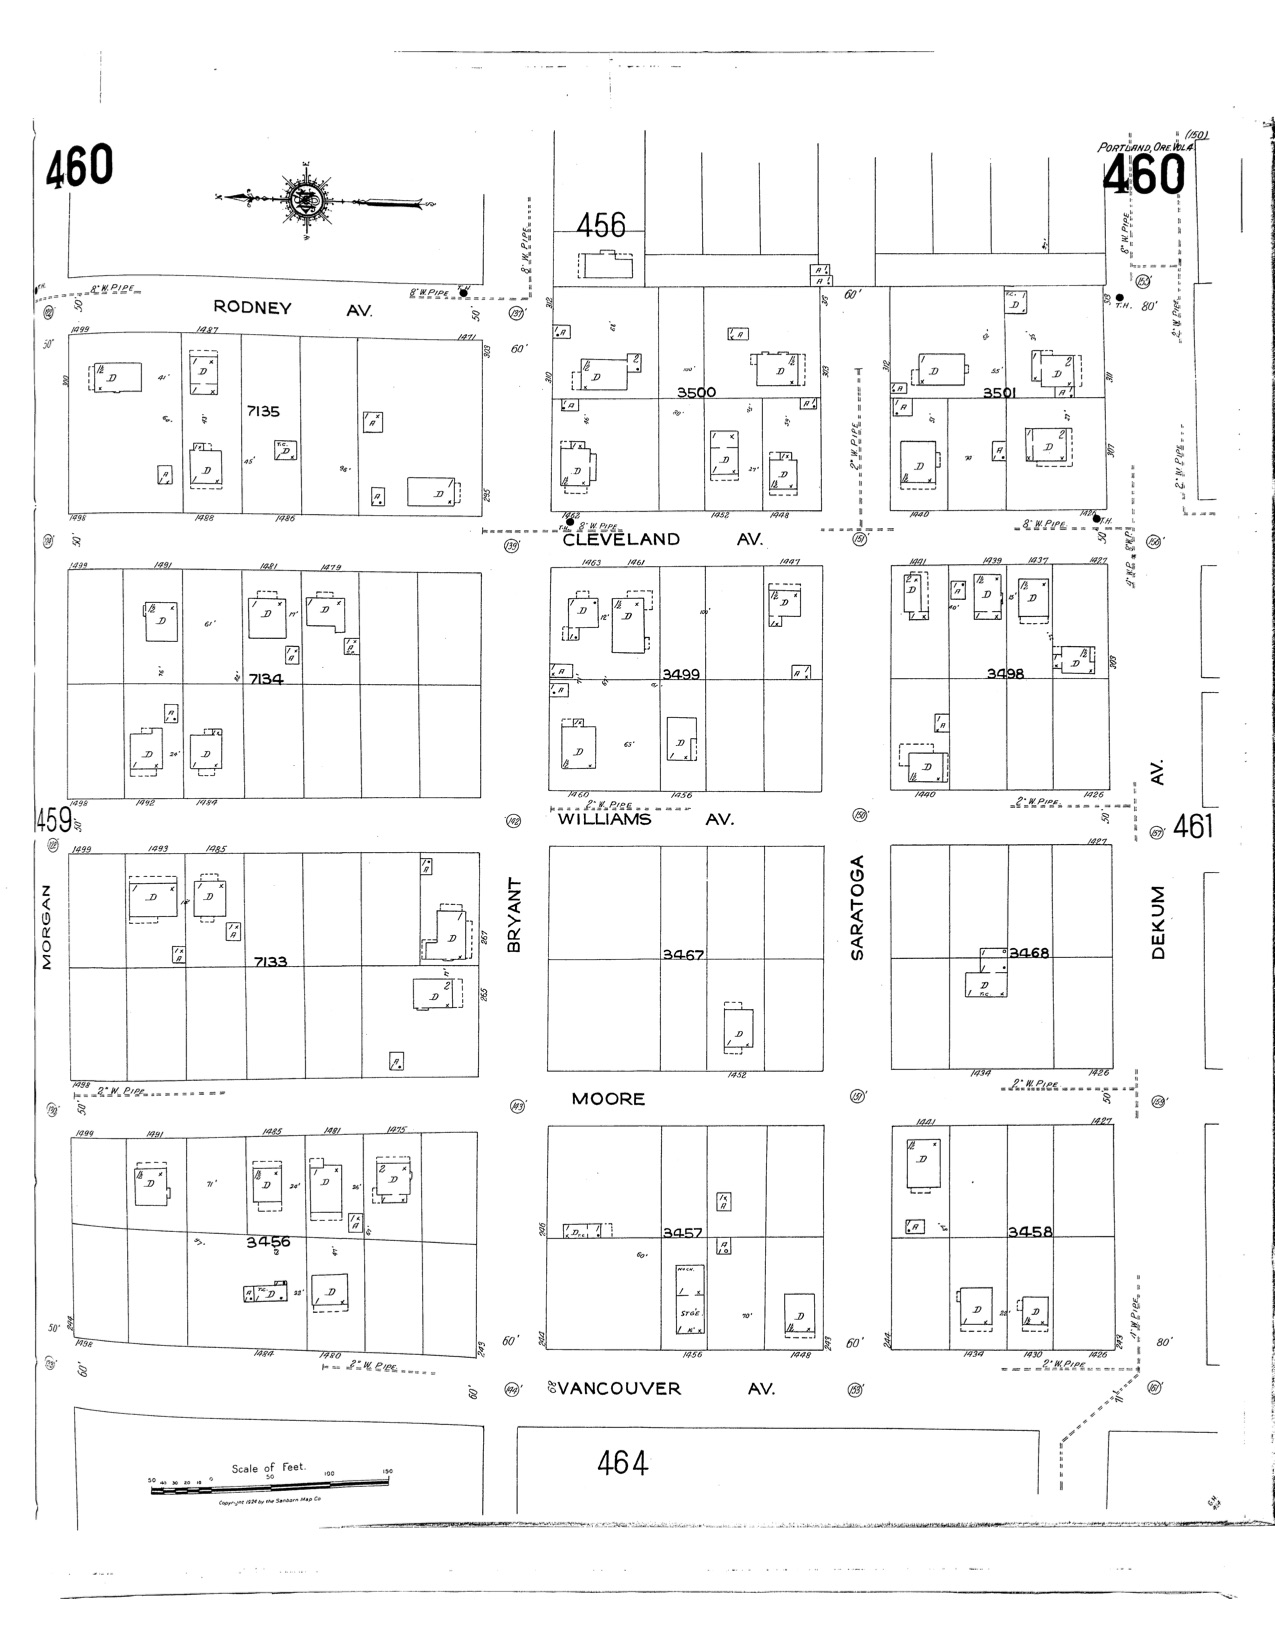
\includegraphics{images/image1.jpg}
\caption{alt\_text}
\end{figure}

\hypertarget{table-of-contents}{%
\subsection{Table of Contents}\label{table-of-contents}}

{[}TOC{]}

\hypertarget{section}{%
\subsection{}\label{section}}

\hypertarget{land}{%
\subsection{Land}\label{land}}

At the time of his death Captain Lewis Love had expanded the original
640 acres of his 1850 donation land claim to 757 acres. The original
claim was bounded by (what is now) Eight Street to the east, the I-5
freeway to the west, the Columbia Slough to the north, and Bryant Street
to the south. The parcels he added, which were part of the original
Switzler donation land claims, were between the Columbia Slough and the
Columbia River. After Lewis Love's death in 1903 the 750+ acres were
divided up among his six children Lewis, Mary, William, Green, Fred, and
Malinda (William and Malinda had died, so their piece of the pie went to
their surviving children). This resulted in six vertical strips of land,
each of about 125 acres, from (what is now) Bryant Street in the south
to the Columbia Slough in the north. In this note we are mainly
interested in the strip between Union Avenue (now MLK) and (what is now)
Rodney Avenue. It went to Mary Love (by that time Mary Stafford).

\hypertarget{section-1}{%
\subsection{}\label{section-1}}

\hypertarget{plats-and-streets}{%
\subsection{Plats and Streets}\label{plats-and-streets}}

It is important to understand that all this land was just land. There
was nothing on it, only scrubs, bushes, and trees. There was, however,
some development to the south (Piedmont Park) and to the east
(Woodlawn). Piedmont Park was platted in 1891 by J.P and Louisa M.
Menefee, F. W. and Ida E. Torgler, and Charles and Emma Woodcock. Here
is the plat map. The strip of land inherited by Mary Stafford starts
directly north of Piedmont Park.

{\textgreater\textgreater\textgreater\textgreater\textgreater{}
gd2md-html alert: inline image link here (to images/image2.png). Store
image on your image server and adjust path/filename/extension if
necessary. }(Back to top)(Next
alert){\textgreater\textgreater\textgreater\textgreater\textgreater{} }

\begin{figure}
\centering
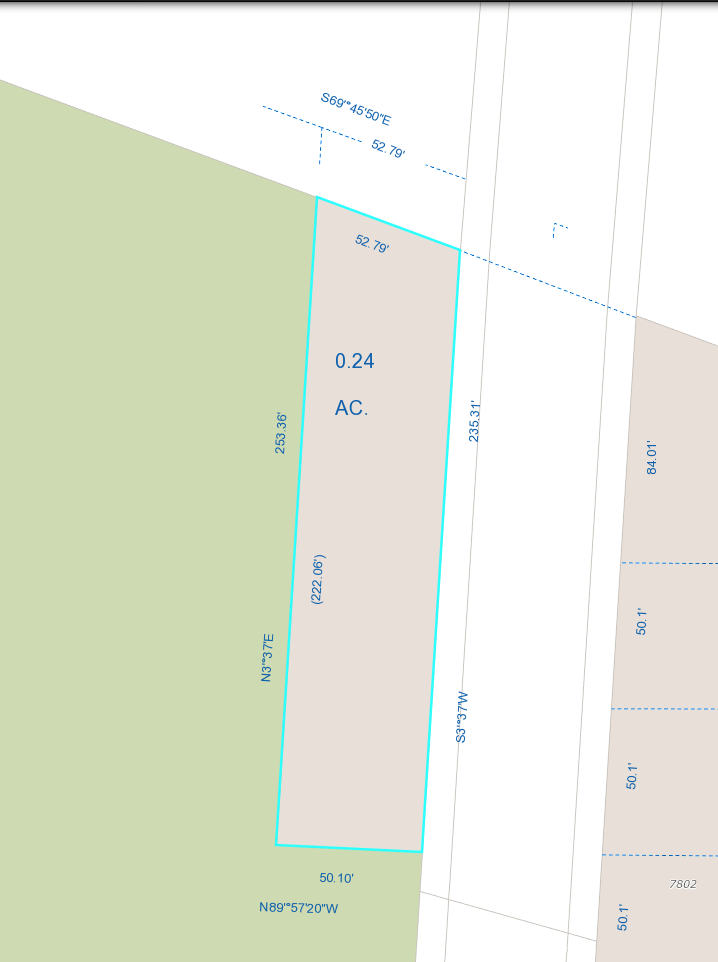
\includegraphics{images/image2.png}
\caption{alt\_text}
\end{figure}

The platting of Piedmont Park happened just before the Great Street
Renaming of January 12, 1892, which was made necessary by the annexation
of Albina and East Portland into the City of Portland. Columbus Avenue
became Dekum Avenue and Margaretta Avenue became Union Avenue. A Street
became Garfield Avenue and B Street became Mallory Street. Woodlawn
Avenue became Woodlawn Street, and Rodney Avenue became Hendricks
Avenue. The new names and the old names are on this map from 1892.

{\textgreater\textgreater\textgreater\textgreater\textgreater{}
gd2md-html alert: inline image link here (to images/image3.png). Store
image on your image server and adjust path/filename/extension if
necessary. }(Back to top)(Next
alert){\textgreater\textgreater\textgreater\textgreater\textgreater{} }

\begin{figure}
\centering
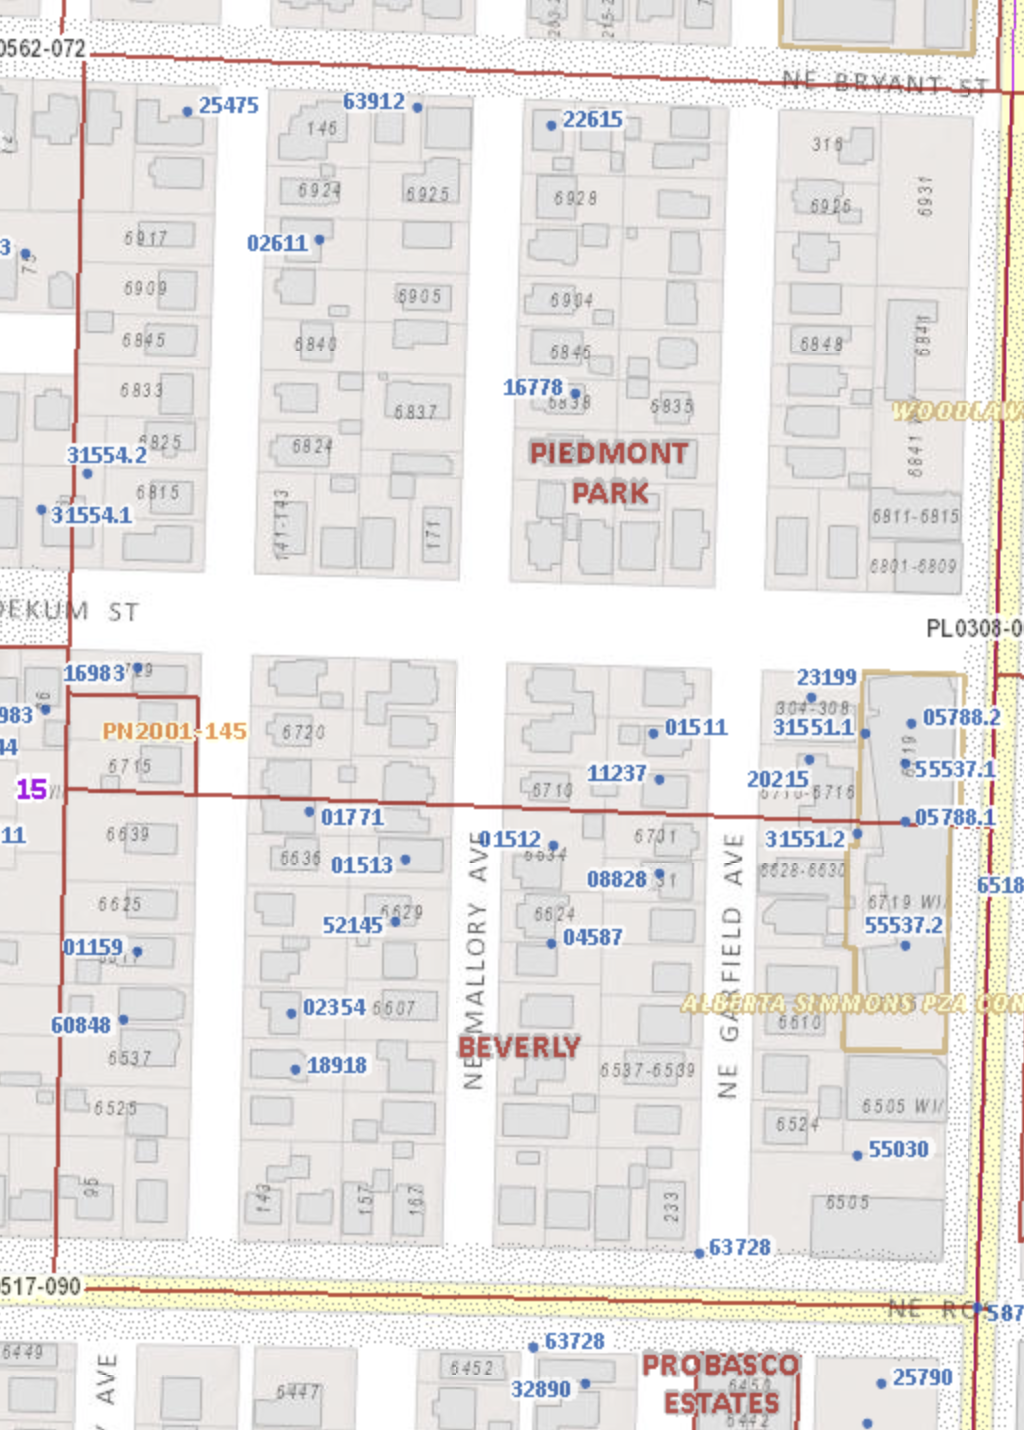
\includegraphics{images/image3.png}
\caption{alt\_text}
\end{figure}

Note that Union Avenue north of Piedmont was not really a street yet,
just the thought of a street. None of the streets in this map were
actually paved, and only a small percentage of the lots in the blocks of
these subdivisions actually had houses. In 1904 Hendricks Avenue became
Rodney Avenue (again !) and in 1907 Woodlawn Street became Bryant
Street.

\hypertarget{section-2}{%
\subsection{}\label{section-2}}

\hypertarget{grid-deviations}{%
\subsection{Grid Deviations}\label{grid-deviations}}

I will take this opportunity to discuss some peculiar deviations from
the grid pattern in the Bryant-Rodney-Saratoga area. Here is a piece of
a Portland Maps.

{\textgreater\textgreater\textgreater\textgreater\textgreater{}
gd2md-html alert: inline image link here (to images/image4.png). Store
image on your image server and adjust path/filename/extension if
necessary. }(Back to top)(Next
alert){\textgreater\textgreater\textgreater\textgreater\textgreater{} }

\begin{figure}
\centering
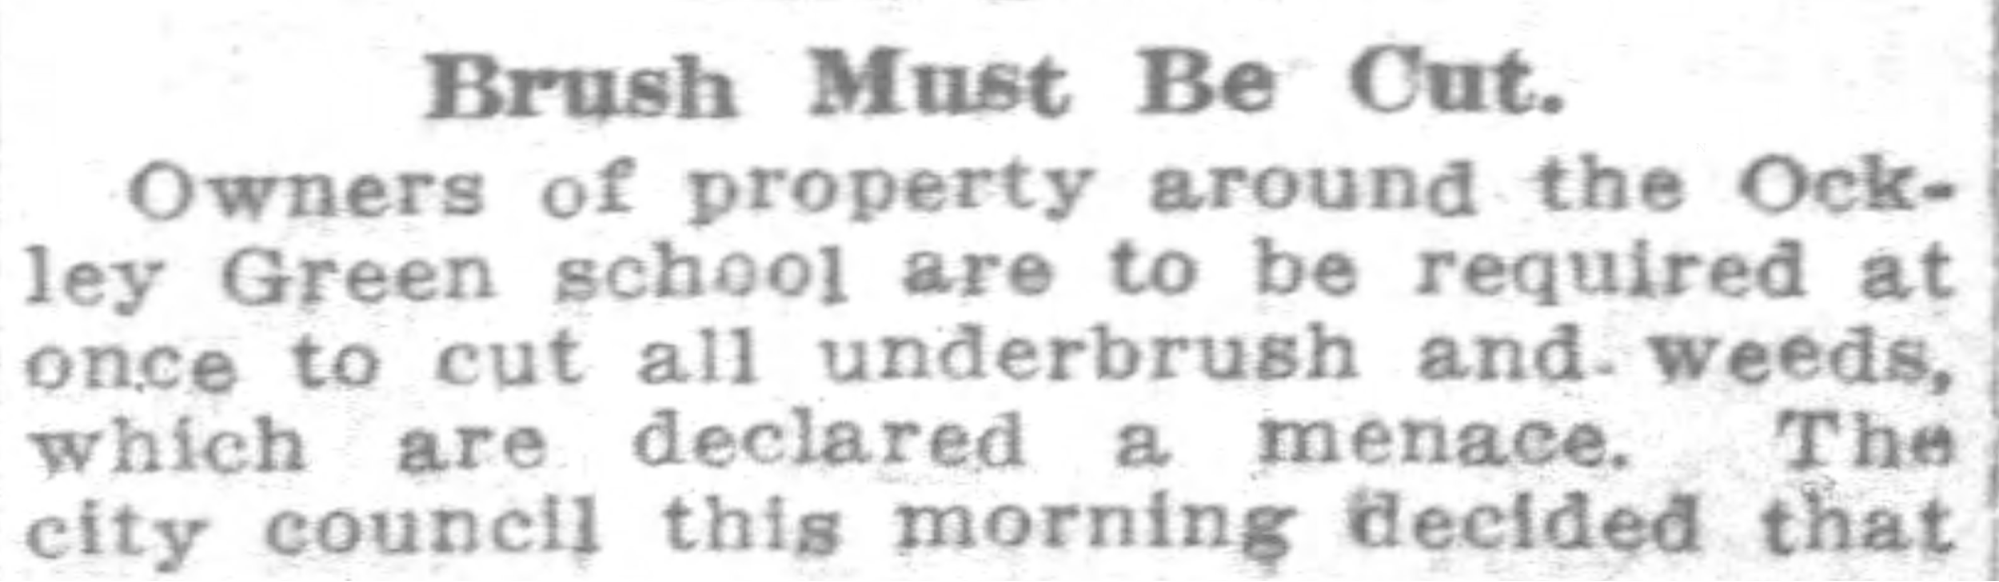
\includegraphics{images/image4.png}
\caption{alt\_text}
\end{figure}

Saratoga dead-ends going east before it reaches Rodney. Going north,
Rodney Avenue seems to end at Bryant Street. It does not really, because
it picks up again one city block to the west. If you go straight north
at Bryant the street continues as Rodney Court, which ends at Morgan.

Saratoga was platted in 1889 by H. C. Wortman, co-owner of the famous
Olds, Wortman \& King department store downtown. The east boundary of
the subdivision is named Albemarle Street, which did not exist at the
time and has never existed. It was consequently ignored by Menefee et
al, when they platted Piedmont Park two years later. In the 1892
renaming Belmont Avenue in Saratoga became Dekum Avenue. Congress Street
became Cleveland Avenue and Windsor Street became Williams Avenue.

{\textgreater\textgreater\textgreater\textgreater\textgreater{}
gd2md-html alert: inline image link here (to images/image5.png). Store
image on your image server and adjust path/filename/extension if
necessary. }(Back to top)(Next
alert){\textgreater\textgreater\textgreater\textgreater\textgreater{} }

\begin{figure}
\centering
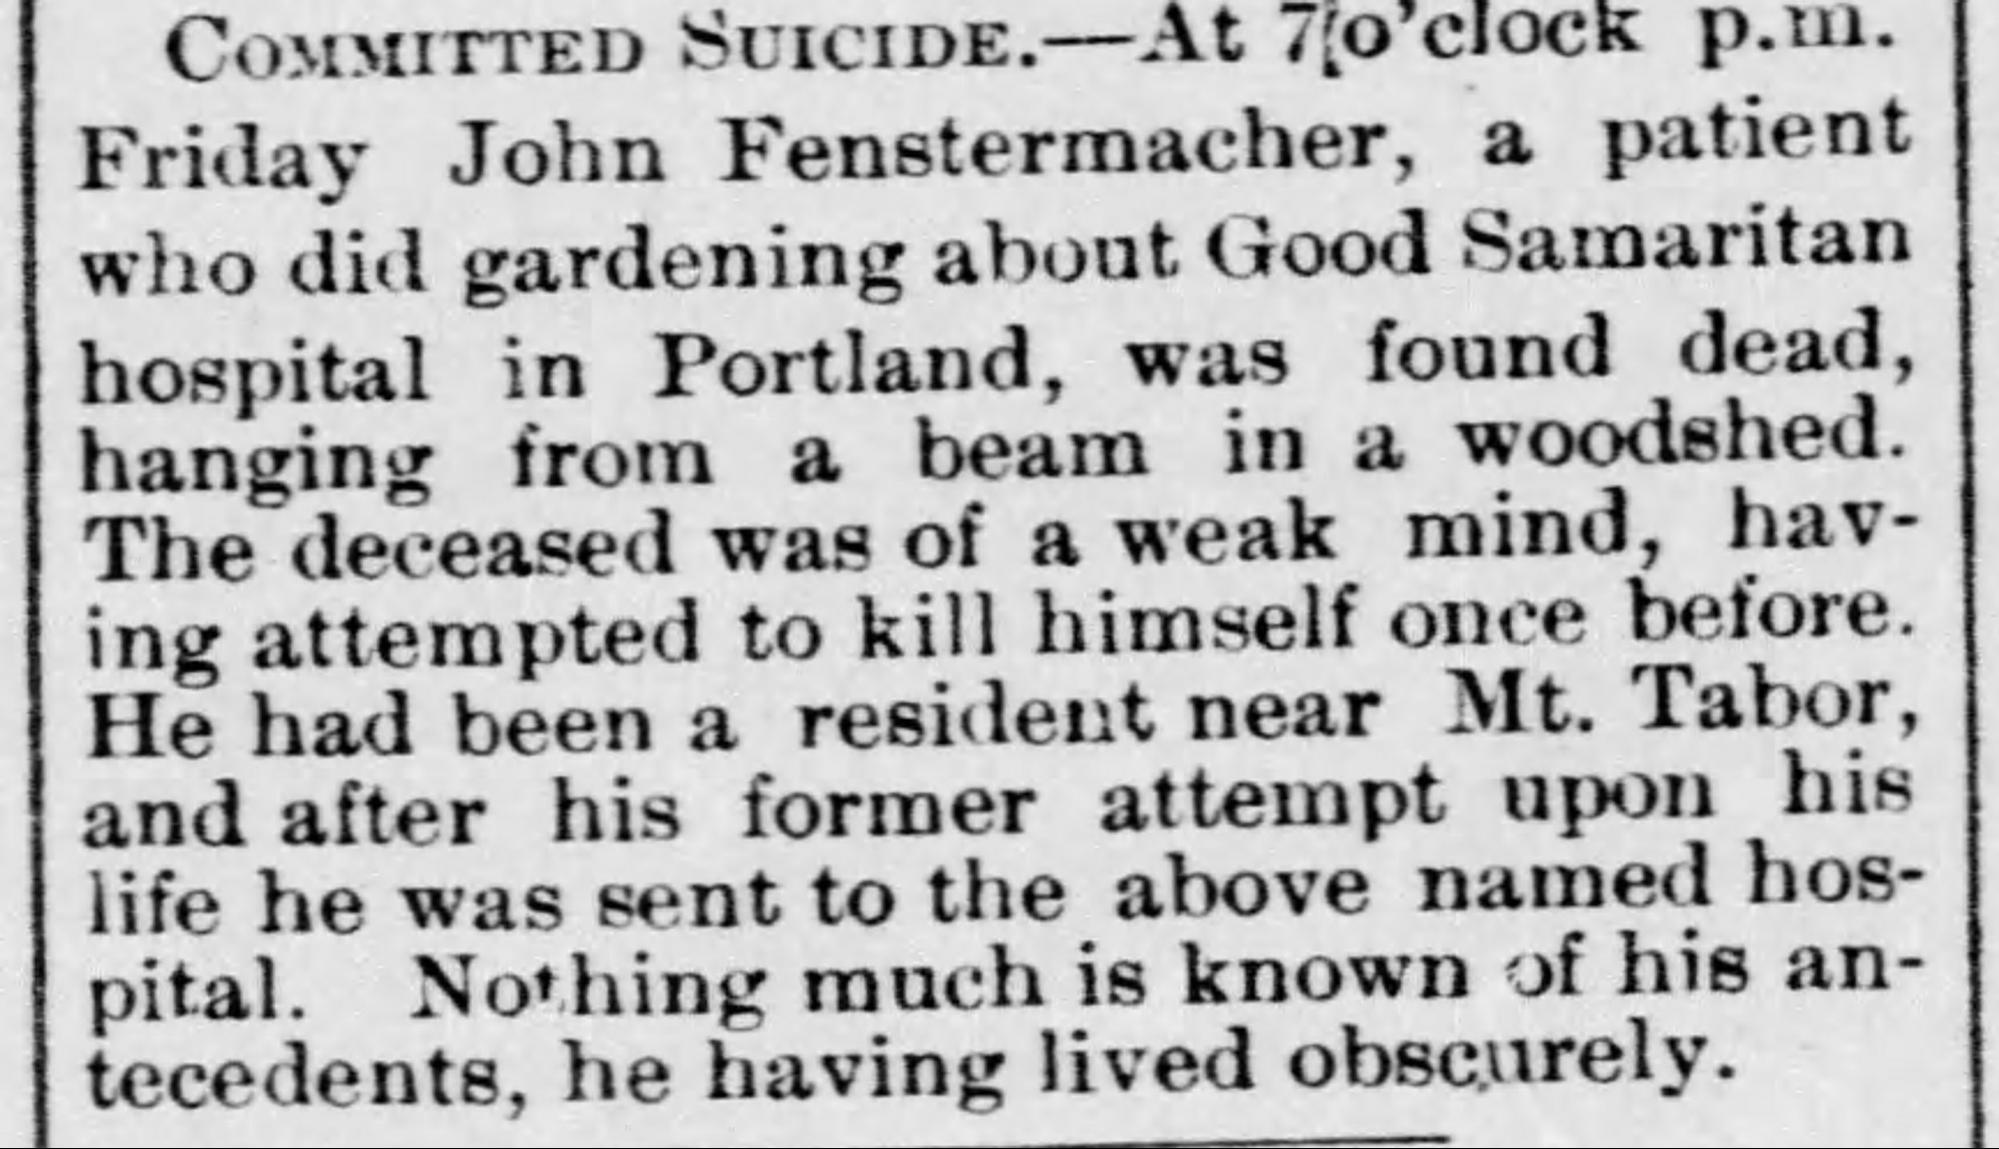
\includegraphics{images/image5.png}
\caption{alt\_text}
\end{figure}

To see what happened with Rodney Avenue, we will look at the plat of
Love's Addition. It was recorded on August 8, 1908 by a whole bunch of
people.

{\textgreater\textgreater\textgreater\textgreater\textgreater{}
gd2md-html alert: inline image link here (to images/image6.png). Store
image on your image server and adjust path/filename/extension if
necessary. }(Back to top)(Next
alert){\textgreater\textgreater\textgreater\textgreater\textgreater{} }

\begin{figure}
\centering
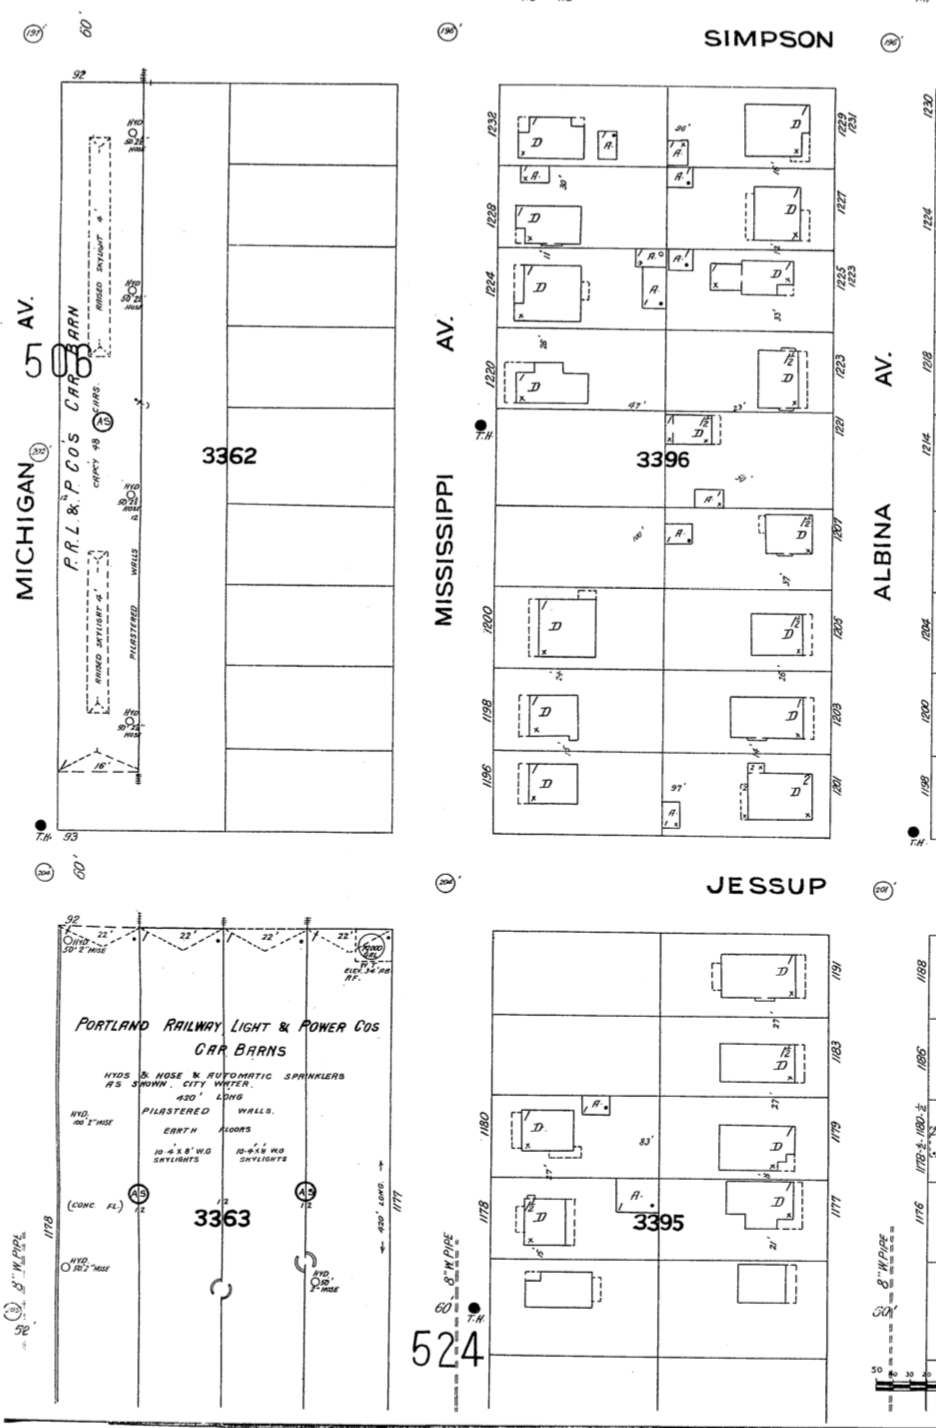
\includegraphics{images/image6.png}
\caption{alt\_text}
\end{figure}

{\textgreater\textgreater\textgreater\textgreater\textgreater{}
gd2md-html alert: inline image link here (to images/image7.png). Store
image on your image server and adjust path/filename/extension if
necessary. }(Back to top)(Next
alert){\textgreater\textgreater\textgreater\textgreater\textgreater{} }

\begin{figure}
\centering
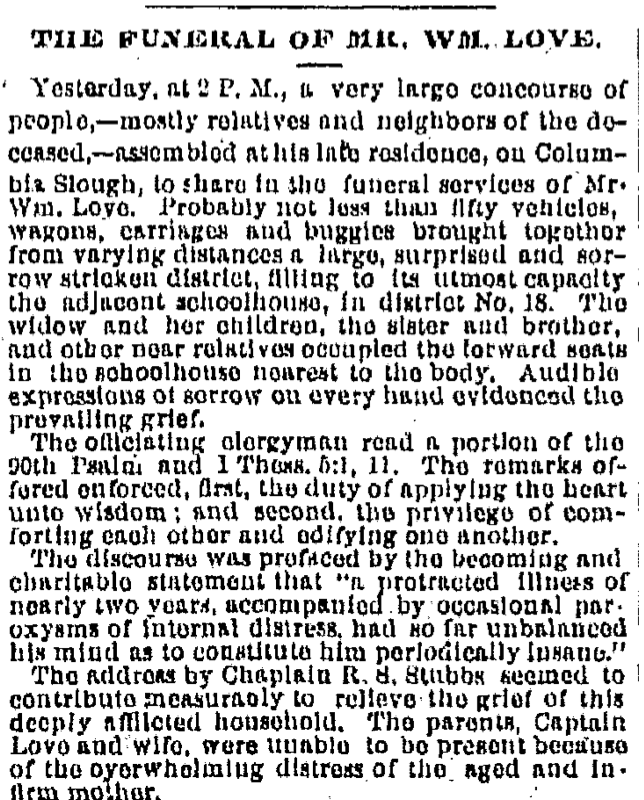
\includegraphics{images/image7.png}
\caption{alt\_text}
\end{figure}

In this list Lewis G. Stafford, Emma J. Walker, Alistress L. Peacher,
Nancy M. Finke, Sarah R. Anderson, Lena G. Richmond, and Sidelia F.
Hohmann were all children of Mary C. Stafford. The Schuldermanns and the
Radkes are not related, afaik. They came into the picture because in
their eagerness to turn the inherited land into money, some pieces of
the land had been sold by the heirs. From the Oregonian of July 21,
1908:

{\textgreater\textgreater\textgreater\textgreater\textgreater{}
gd2md-html alert: inline image link here (to images/image8.png). Store
image on your image server and adjust path/filename/extension if
necessary. }(Back to top)(Next
alert){\textgreater\textgreater\textgreater\textgreater\textgreater{} }

\begin{figure}
\centering
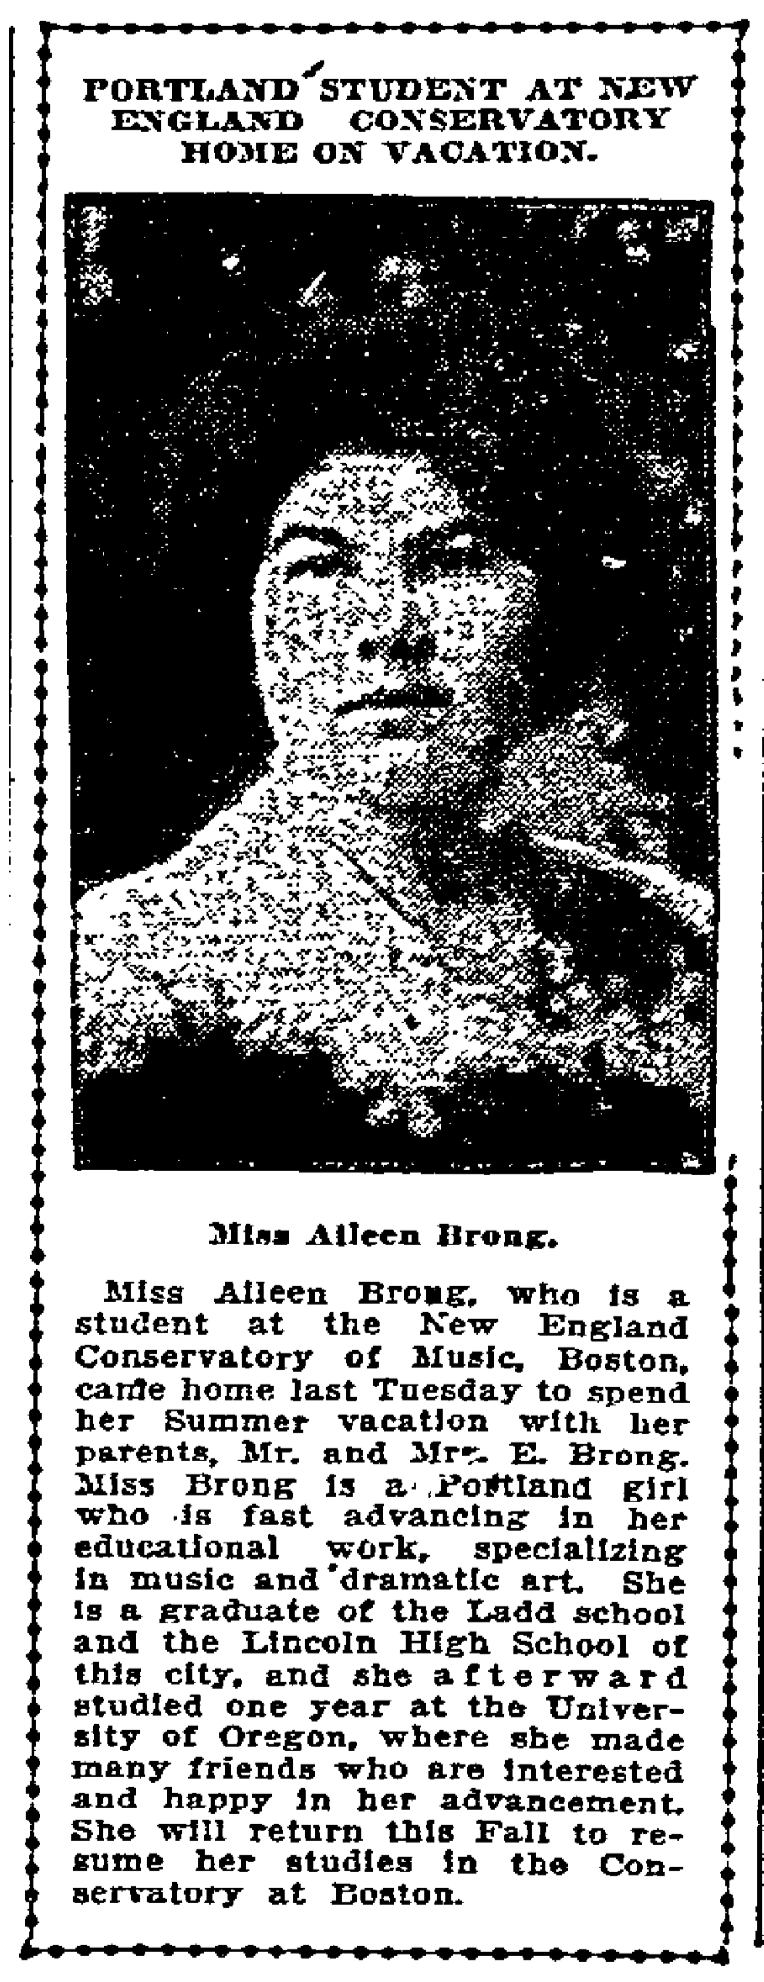
\includegraphics{images/image8.png}
\caption{alt\_text}
\end{figure}

The following map shows the southern part of Love's Addition.

{\textgreater\textgreater\textgreater\textgreater\textgreater{}
gd2md-html alert: inline image link here (to images/image9.png). Store
image on your image server and adjust path/filename/extension if
necessary. }(Back to top)(Next
alert){\textgreater\textgreater\textgreater\textgreater\textgreater{} }

\begin{figure}
\centering
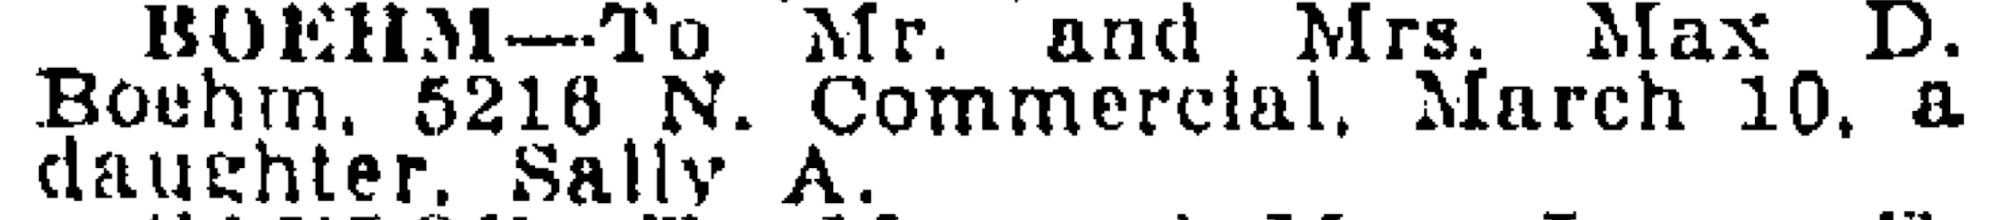
\includegraphics{images/image9.png}
\caption{alt\_text}
\end{figure}

We now see the problem with Rodney Avenue. North of Bryant Street it
forms the border between Love's Addition and Loveleigh, which was
platted around the same time. South of Bryant Street, Rodney Avenue
comes up through the existing subdivision of Piedmont Park, slightly
east of the boundary of Love's Addition and Loveleigh. Putting in Camden
Street did not really solve the problem, and Camden Street was renamed
to Rodney Court in 1922, and to NE Rodney Court in the Great Renumbering
of 1932. The 1932 change thus merely added the NE to the name (as it did
to all streets in the area).

\hypertarget{bryant-area-lots}{%
\subsection{Bryant Area Lots}\label{bryant-area-lots}}

Obviously the purpose of plat a subdivision is to create lots, which
eventually must be sold. It seems that the Stafford family divided the
lots in Love's Addition amongst the many individuals, family or not, who
recorded the plat. In the sequel we shall concentrate on Block 19, lots
7-9, which is a fairly large parcel of 14,407 square feet. It fell to
Sidelia Frances Hohmann. We know this because The Oregon Daily Journal
of August 25, 1913 has a list of all those people in Multnomah County
who are in arrears on their property taxes. The two Stafford sisters
mentioned did not pay for their lots in Love's Addition, and lots 7-9 in
block 19 are in Sidelia's name.

{\textgreater\textgreater\textgreater\textgreater\textgreater{}
gd2md-html alert: inline image link here (to images/image10.png). Store
image on your image server and adjust path/filename/extension if
necessary. }(Back to top)(Next
alert){\textgreater\textgreater\textgreater\textgreater\textgreater{} }

\begin{figure}
\centering
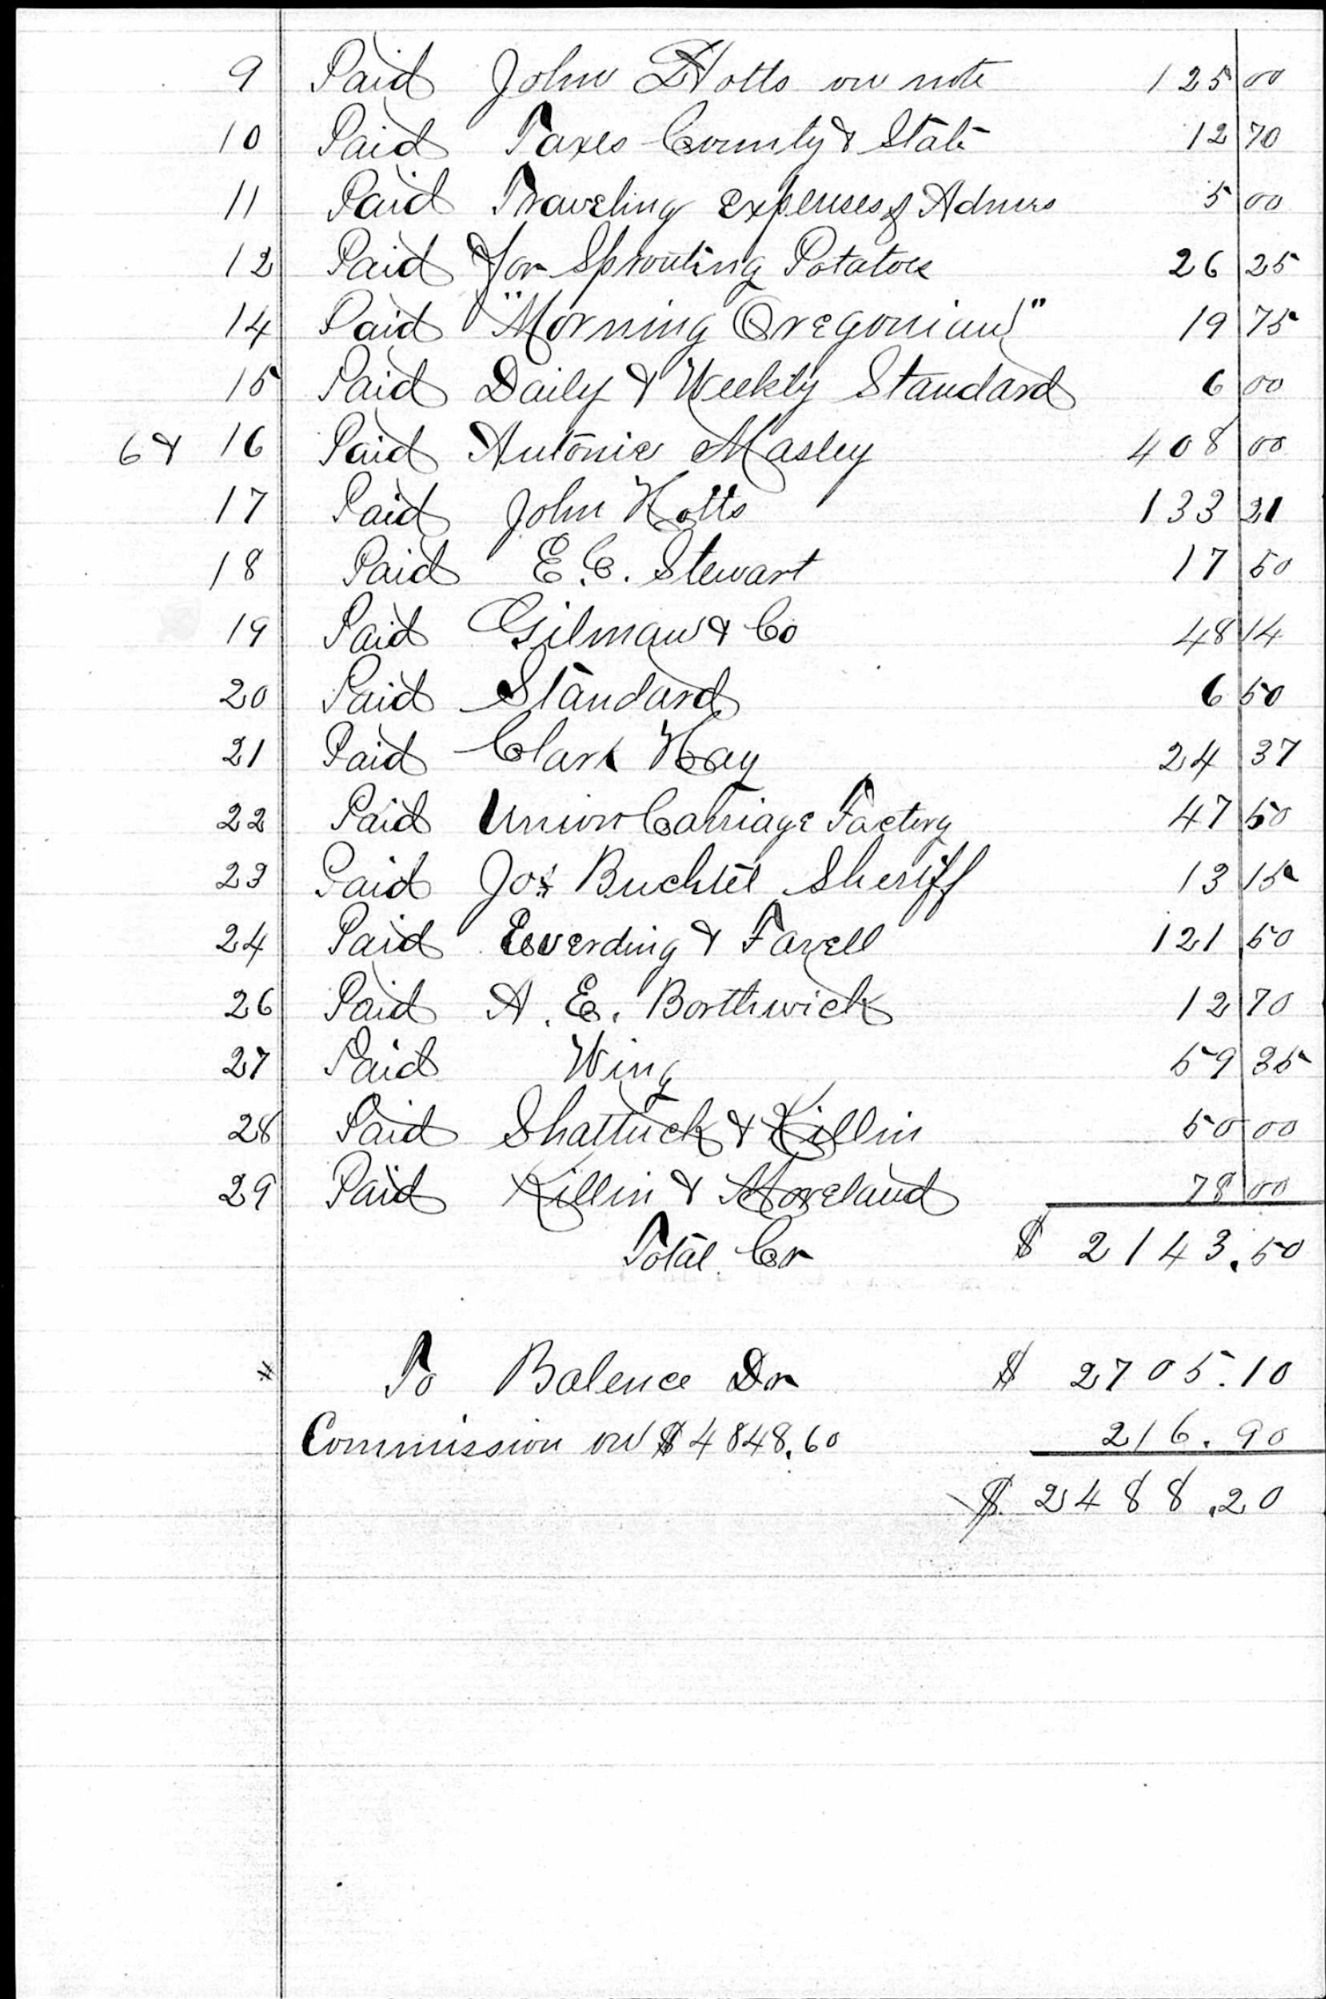
\includegraphics{images/image10.png}
\caption{alt\_text}
\end{figure}

Next, we want to find out if these three lots actually had a house or
houses on it. We can approach this from the present and from the past.
Portland Maps tells us that there is now a house on these three lots,
which are still a single parcel, with street address 107 NE Bryant
Street. If we look at resources from the past we unfortunately cannot
use the 1907 Portland Block Book, because it only covers platted
subdivisions, and Love's Addition was not platted yet. This is
unfortunate, because the Block Book would tell us for each lot who owned
it in 1906. It does not tell us if there was actually a house on the
lot. For that we need the Sanborn maps. Again, unfortunately, the 1908
Sanborn maps do not really cover the area north of Bryant, probably
because there was not yet any development there. Nothing to insure for
Sanborn. Nevertheless, here it is. The structure on the northwest corner
of Rodney and Bryant may be some water tower or fire lookout.

{\textgreater\textgreater\textgreater\textgreater\textgreater{}
gd2md-html alert: inline image link here (to images/image11.png). Store
image on your image server and adjust path/filename/extension if
necessary. }(Back to top)(Next
alert){\textgreater\textgreater\textgreater\textgreater\textgreater{} }

\begin{figure}
\centering
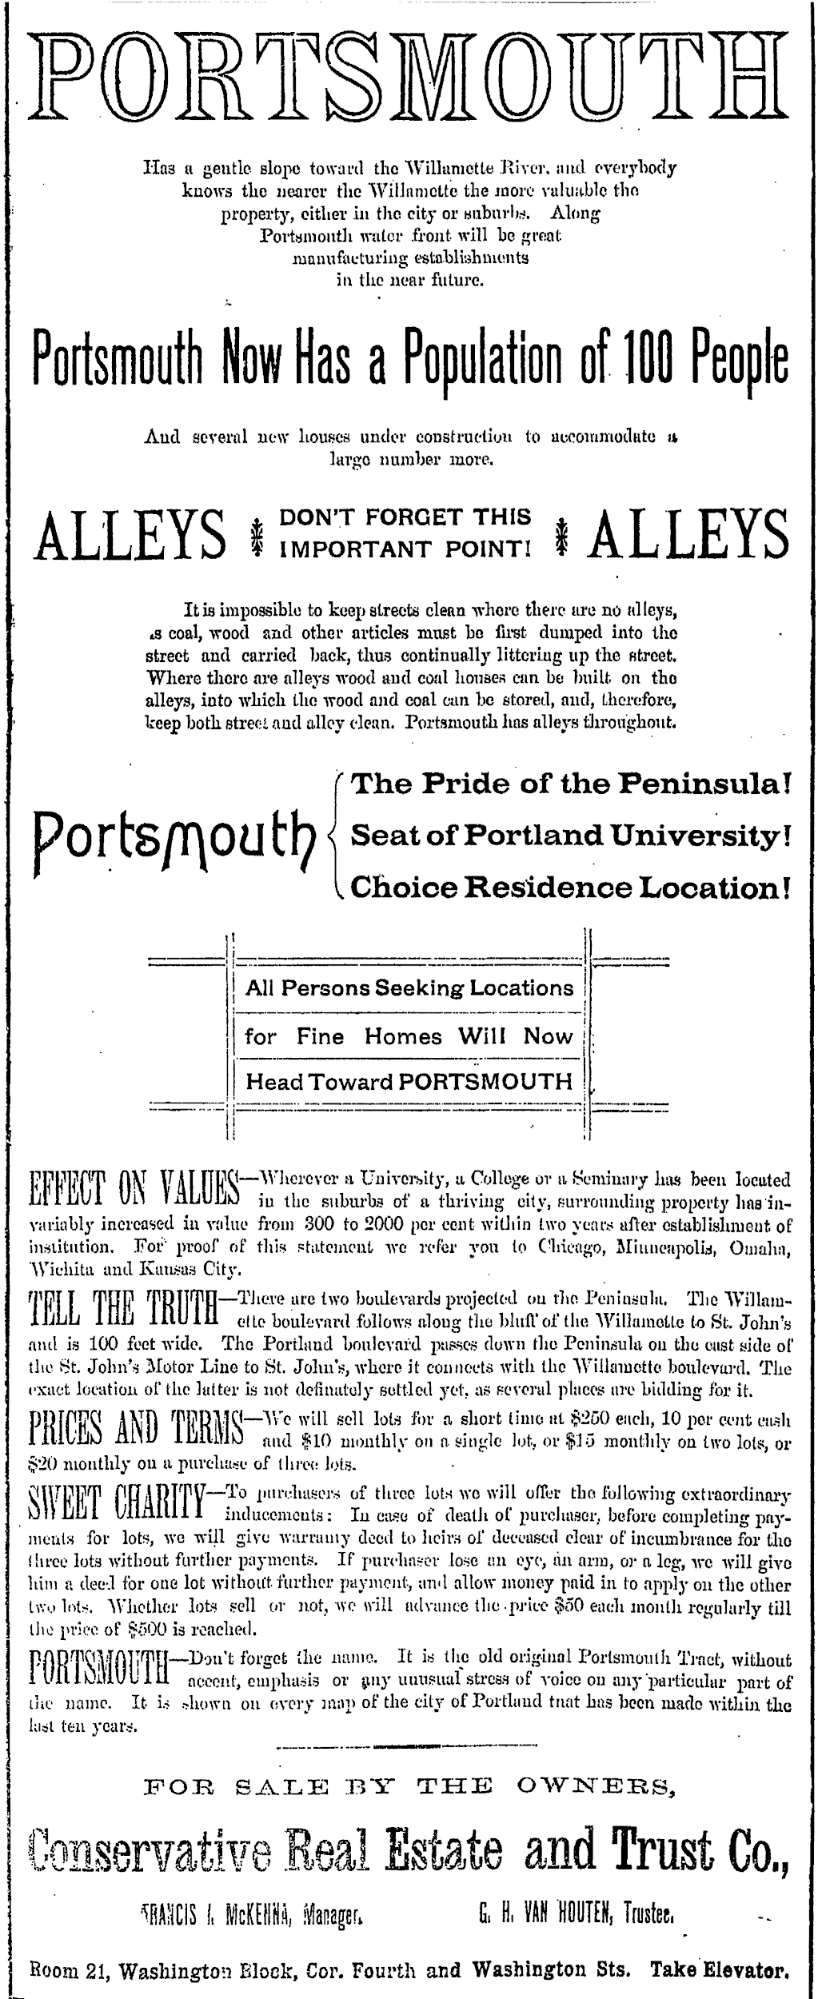
\includegraphics{images/image11.png}
\caption{alt\_text}
\end{figure}

Sanborn map number 456 from 1924 is pretty clear, however.

{\textgreater\textgreater\textgreater\textgreater\textgreater{}
gd2md-html alert: inline image link here (to images/image12.jpg). Store
image on your image server and adjust path/filename/extension if
necessary. }(Back to top)(Next
alert){\textgreater\textgreater\textgreater\textgreater\textgreater{} }

\begin{figure}
\centering
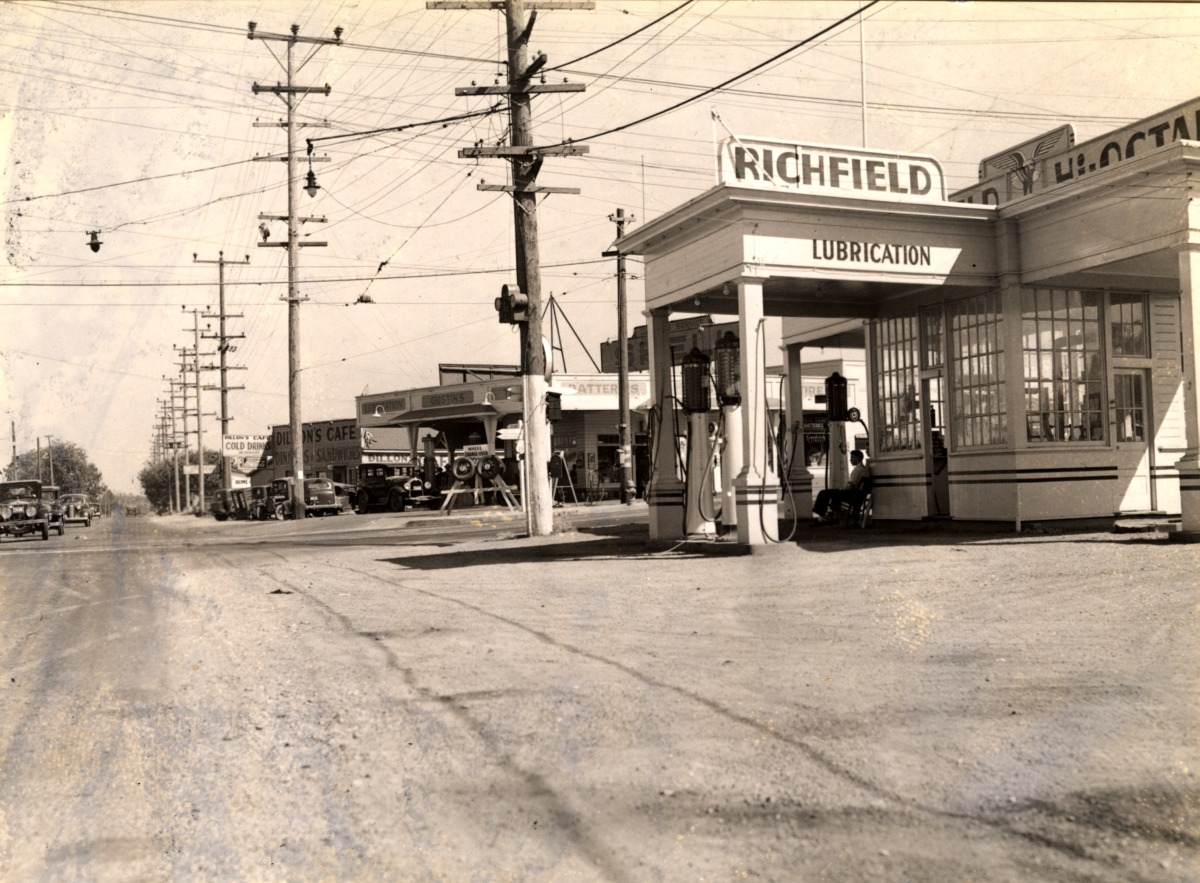
\includegraphics{images/image12.jpg}
\caption{alt\_text}
\end{figure}

There is a house on the three lots, the same house as shown on Portland
Maps, with street address 311 Bryant Street. The Great Renumbering of
1932 documents show that 311 Bryant Street did indeed become 107 NE
Bryant Street.

{\textgreater\textgreater\textgreater\textgreater\textgreater{}
gd2md-html alert: inline image link here (to images/image13.png). Store
image on your image server and adjust path/filename/extension if
necessary. }(Back to top)(Next
alert){\textgreater\textgreater\textgreater\textgreater\textgreater{} }

\begin{figure}
\centering
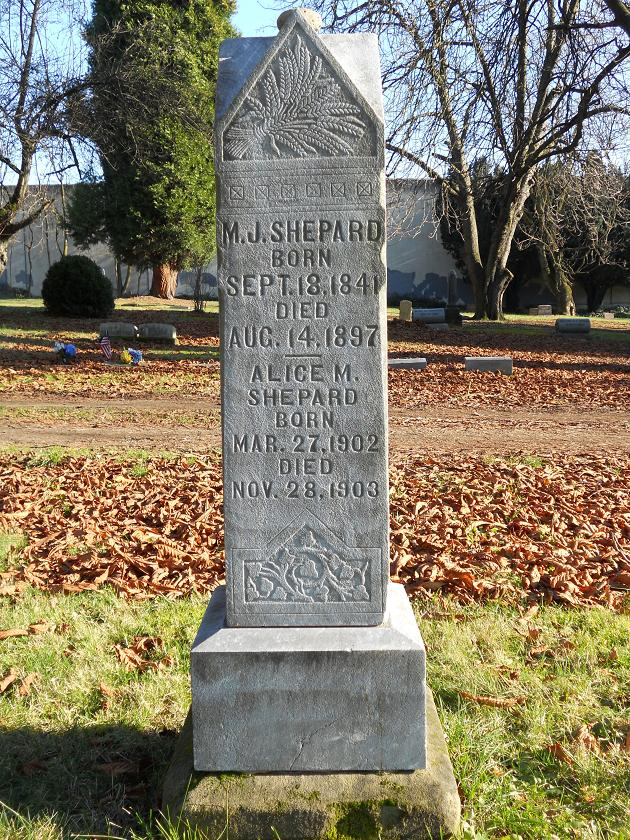
\includegraphics{images/image13.png}
\caption{alt\_text}
\end{figure}

Next question. Who built the house and when ? In the Oregon Daily
Journal of September 1, 1909 we see a building permit issued to E. J.
Price.

{\textgreater\textgreater\textgreater\textgreater\textgreater{}
gd2md-html alert: inline image link here (to images/image14.png). Store
image on your image server and adjust path/filename/extension if
necessary. }(Back to top)(Next
alert){\textgreater\textgreater\textgreater\textgreater\textgreater{} }

\begin{figure}
\centering
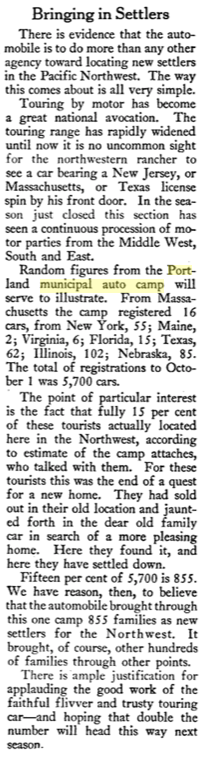
\includegraphics{images/image14.png}
\caption{alt\_text}
\end{figure}

No misunderstanding is possible -- there is only one parcel between
Rodney and Camden. Portland Maps also tells us the house was built in
1909. Now who was E. J. Price, and how was he/she related to Sidelia
Hohmann ?

\hypertarget{section-3}{%
\subsection{}\label{section-3}}

\hypertarget{sidelia-stafford-hohmann-price-thode}{%
\subsection{Sidelia
Stafford-Hohmann-Price-Thode}\label{sidelia-stafford-hohmann-price-thode}}

First, something about Sidelia Stafford, who went by Delia when she was
young. She was born February 22, 1876, and thus was 33 years old in
1909. We can track her through the various federal censuses and city
directories. Delia Stafford in the 1880 census is 5 years old and lives
at home in the Grant district with her carpenter father, her mother, and
her six siblings. In the 1893 city directory Delia Stafford was a
domestic, living on 353 First Street. But then something happened. In
1896 Delia married George A. Hohmann, a Canadian citizen working as a
tin smith or sheet metal worker, and she moved to Astoria. The 1900
census shows her living with George and their two daughters Irene and
Alice on Commercial Street in Astoria, in some sort of boarding house or
hotel, run by one Palomina Teal. The marriage does not last. Delia moved
back to Portland, and in 1907-1908 she lived at the parental home on 325
E. 7th Street. She placed an advertisement in the Oregonian of February
26, 1905.

{\textgreater\textgreater\textgreater\textgreater\textgreater{}
gd2md-html alert: inline image link here (to images/image15.png). Store
image on your image server and adjust path/filename/extension if
necessary. }(Back to top)(Next
alert){\textgreater\textgreater\textgreater\textgreater\textgreater{} }

\begin{figure}
\centering
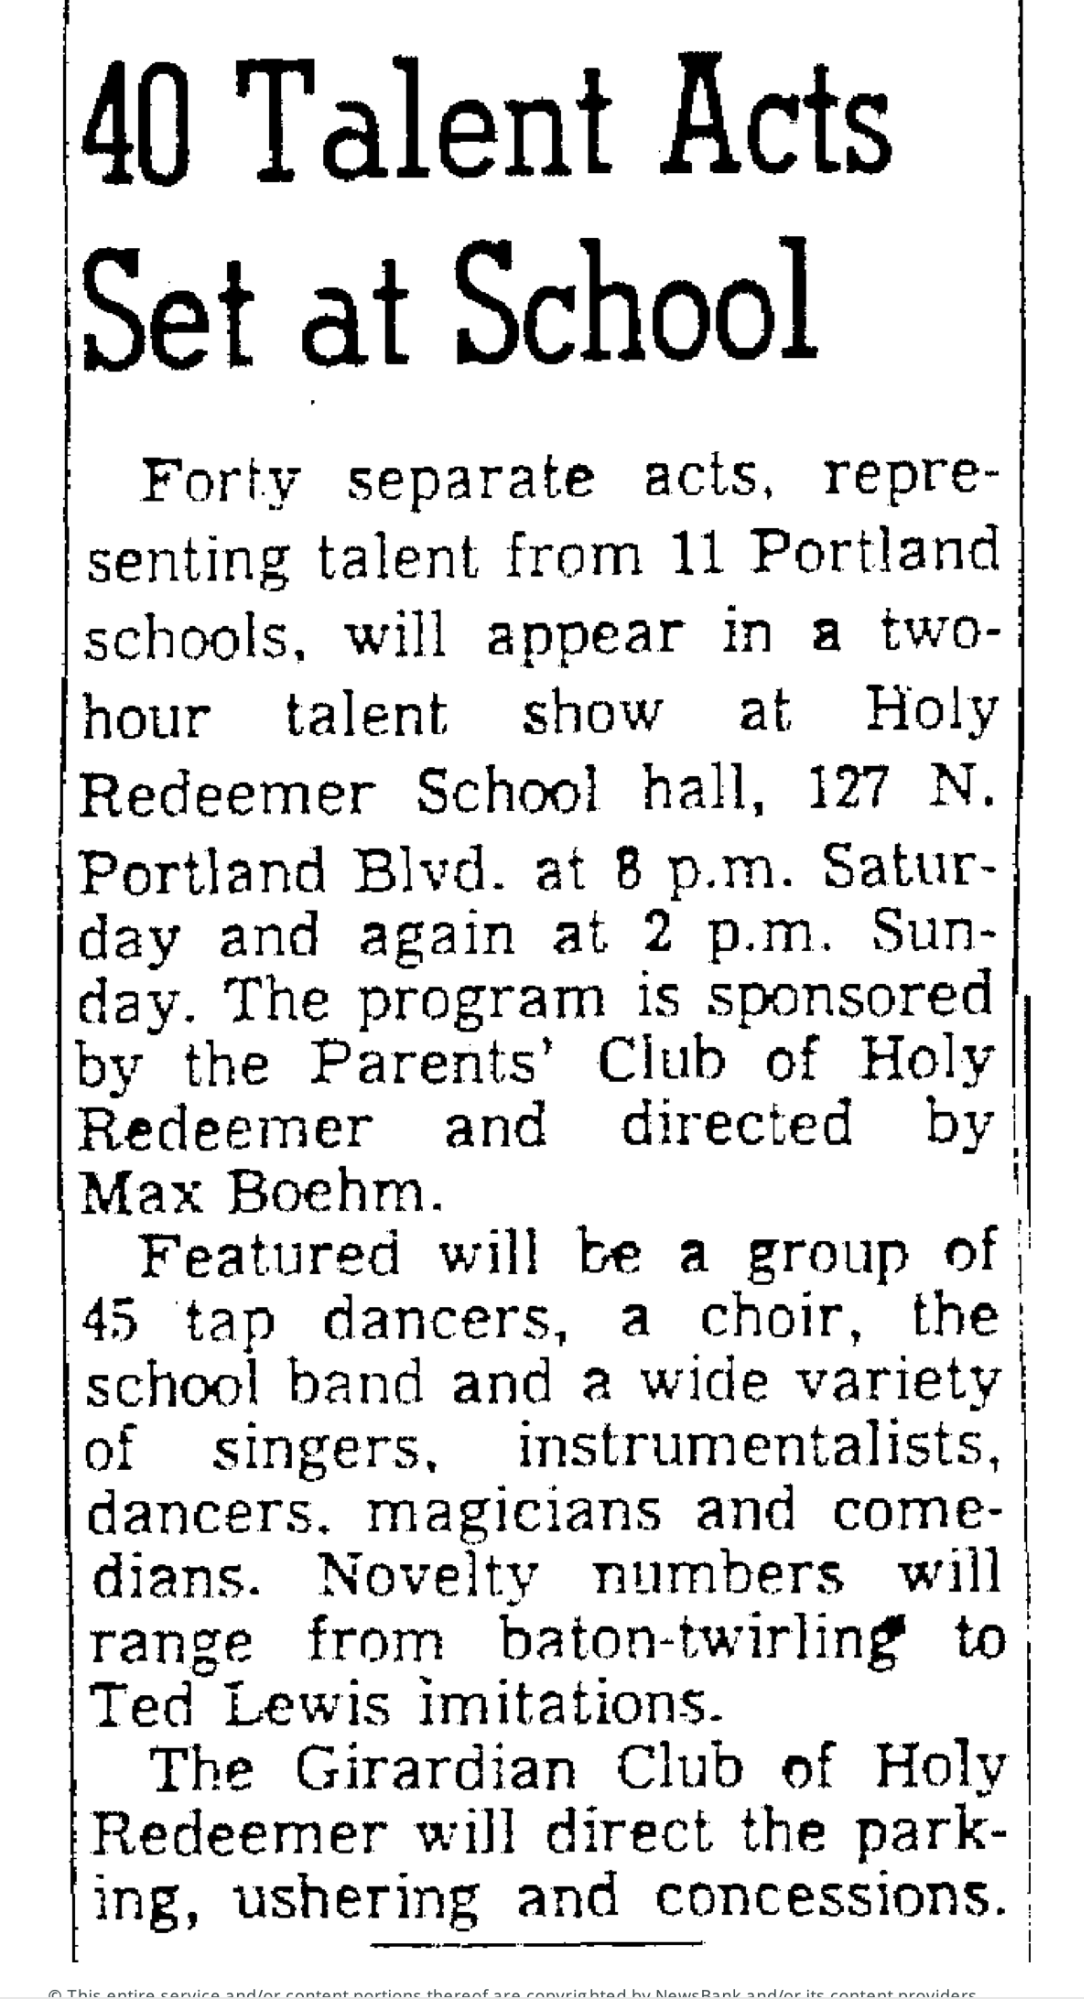
\includegraphics{images/image15.png}
\caption{alt\_text}
\end{figure}

And, not much later, the Oregonian of January 27, 1907 lets us know she
filed for divorce.

{\textgreater\textgreater\textgreater\textgreater\textgreater{}
gd2md-html alert: inline image link here (to images/image16.png). Store
image on your image server and adjust path/filename/extension if
necessary. }(Back to top)(Next
alert){\textgreater\textgreater\textgreater\textgreater\textgreater{} }

\begin{figure}
\centering
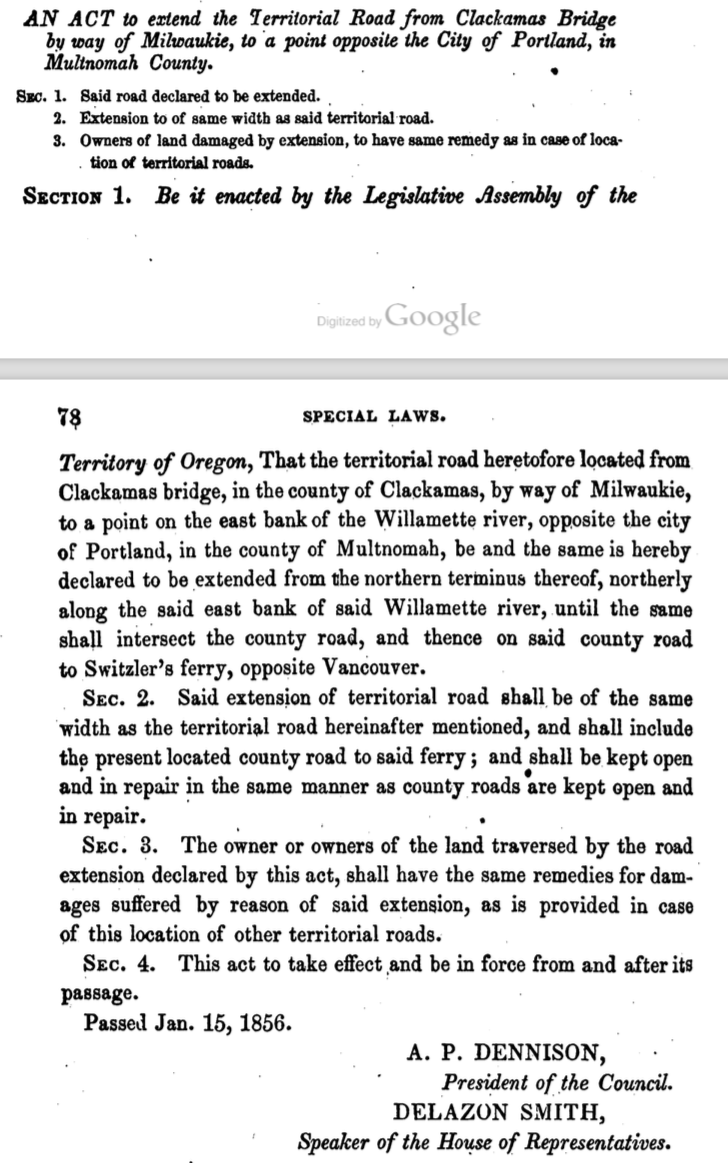
\includegraphics{images/image16.png}
\caption{alt\_text}
\end{figure}

It is of some interest that in the Portland City Directories, all the
way until 1927, she remains listed as Sidelia F. Hohmann, widow of
George A. Hohmann. In the meantime, however, George marries Katie Dreger
in June of 1908 and definitely does not die until 1953.

Delia now marries Elijah Price on July 31, 1908. This is obviously the
E. J. Price of the building permit. Indeed, the 1910 census shows Elijah
and Sidelia Price, with children Irene, Alice, and Walter, living at a
house with address 311 Rodney (a mistake by the census taker). The
second marriage goes the way of the first. The Oregonian of June 17,
1911 reports the divorce.

{\textgreater\textgreater\textgreater\textgreater\textgreater{}
gd2md-html alert: inline image link here (to images/image17.png). Store
image on your image server and adjust path/filename/extension if
necessary. }(Back to top)(Next
alert){\textgreater\textgreater\textgreater\textgreater\textgreater{} }

\begin{figure}
\centering
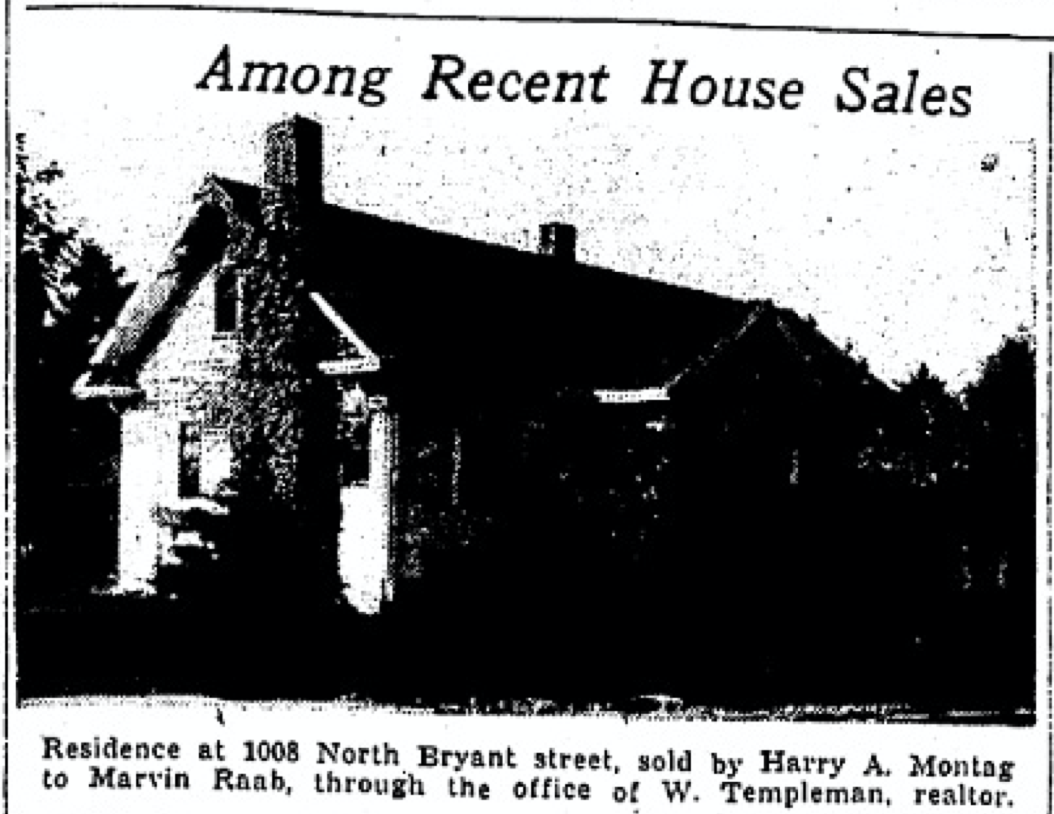
\includegraphics{images/image17.png}
\caption{alt\_text}
\end{figure}

On May 3, 1918 Delia, now 42, married 33 year old Ernest August Thode, a
ship filler, if I read the license correctly. This turns out to be a
really short marriage. The Oregonian of September 23, 1918 let us know
she filed for divorce.

{\textgreater\textgreater\textgreater\textgreater\textgreater{}
gd2md-html alert: inline image link here (to images/image18.png). Store
image on your image server and adjust path/filename/extension if
necessary. }(Back to top)(Next
alert){\textgreater\textgreater\textgreater\textgreater\textgreater{} }

\begin{figure}
\centering
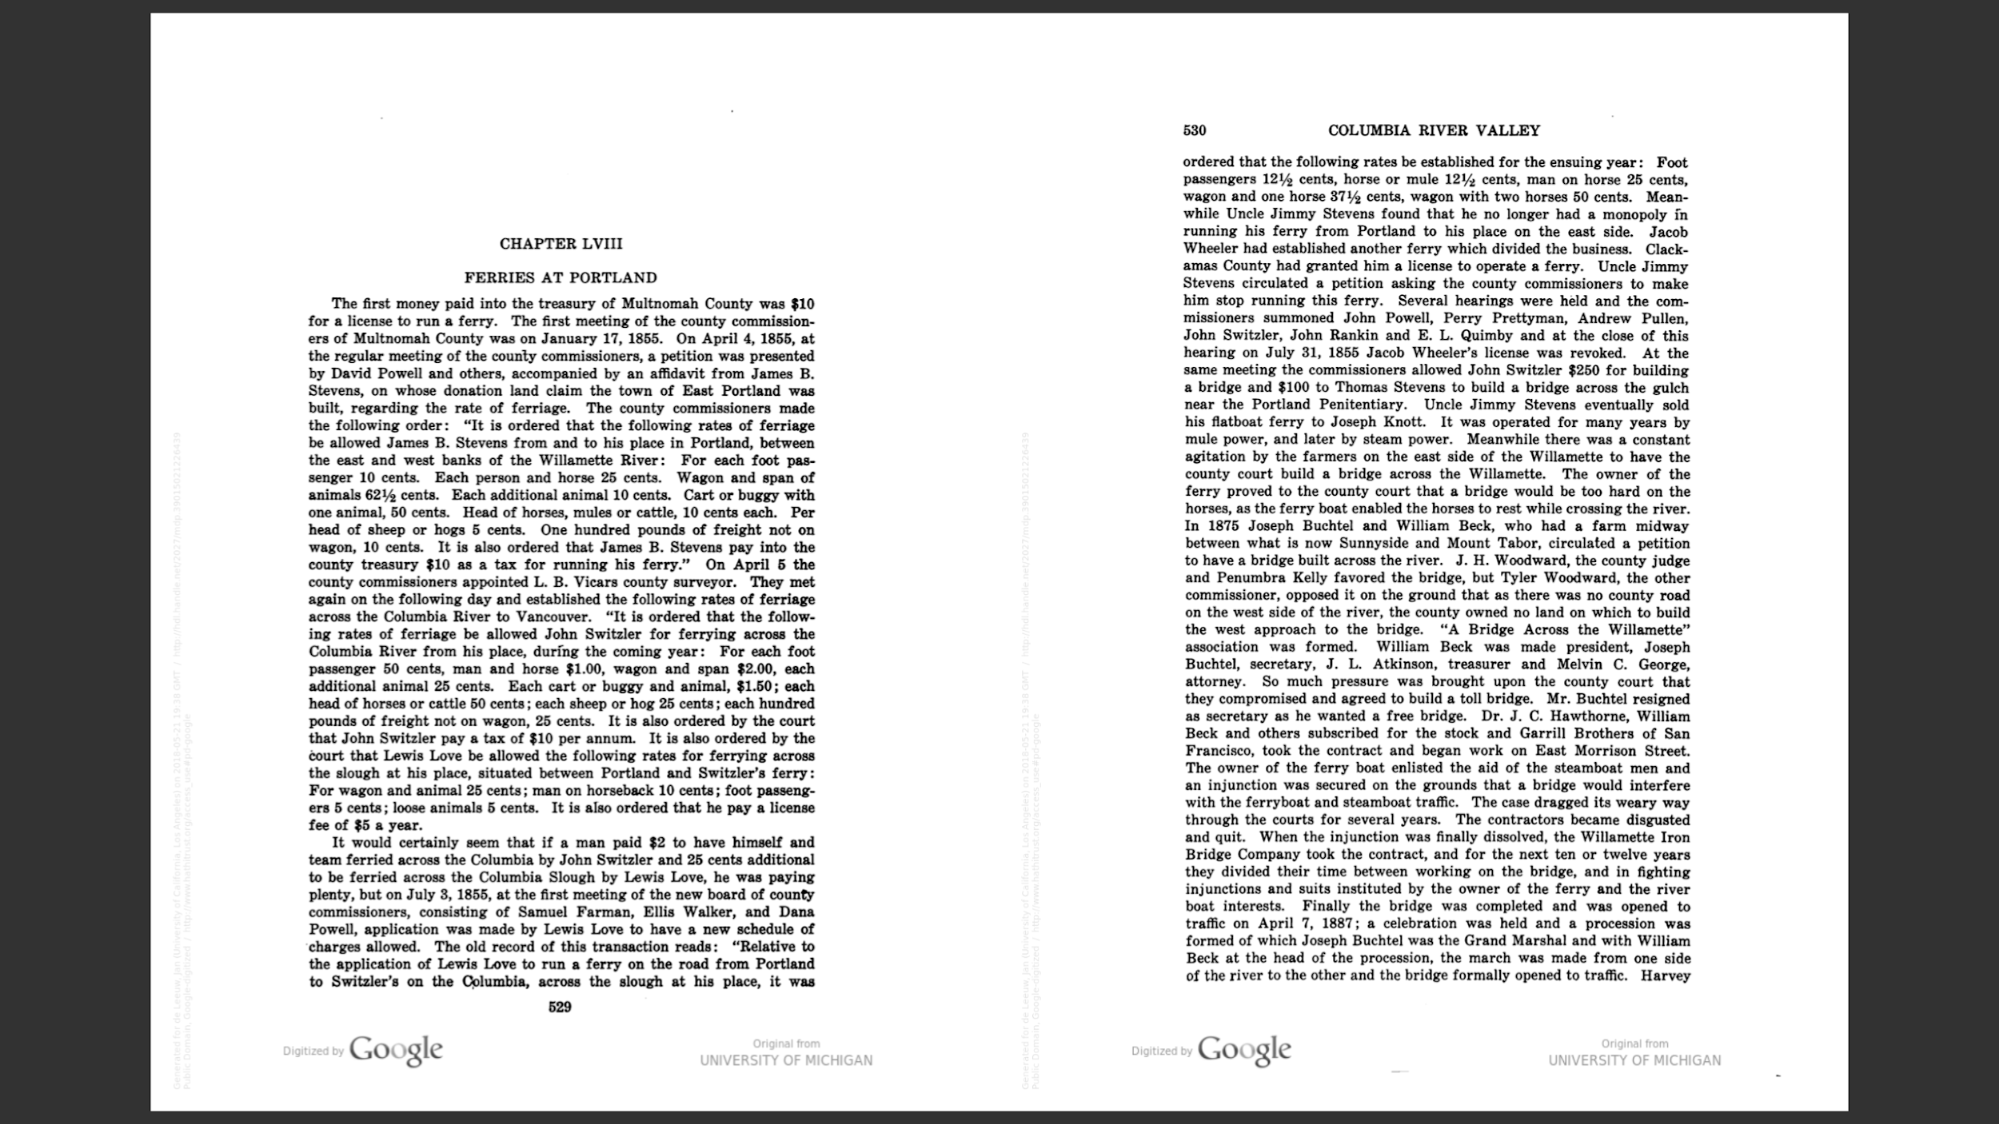
\includegraphics{images/image18.png}
\caption{alt\_text}
\end{figure}

So in the 1920 census we found Sidelia Thode at 311 E. Bryant Street.
Daughter Alice, now 20, still lives at home, and the house is shared
with three male lodgers. In the city directories we find Delia still
living at 311 Bryant in 1910, 1917, 1924 1927, and 1929. Then there is a
gap. I cannot find her in the 1930 census, but in the 1940 census, at
age 64, she lives at 341 SW Meade Street in the house of her daughter
Irene (then Irene Swaggert). On July 1, 1955 the Oregonian published a
cute picture.

{\textgreater\textgreater\textgreater\textgreater\textgreater{}
gd2md-html alert: inline image link here (to images/image19.png). Store
image on your image server and adjust path/filename/extension if
necessary. }(Back to top)(Next
alert){\textgreater\textgreater\textgreater\textgreater\textgreater{} }

\begin{figure}
\centering
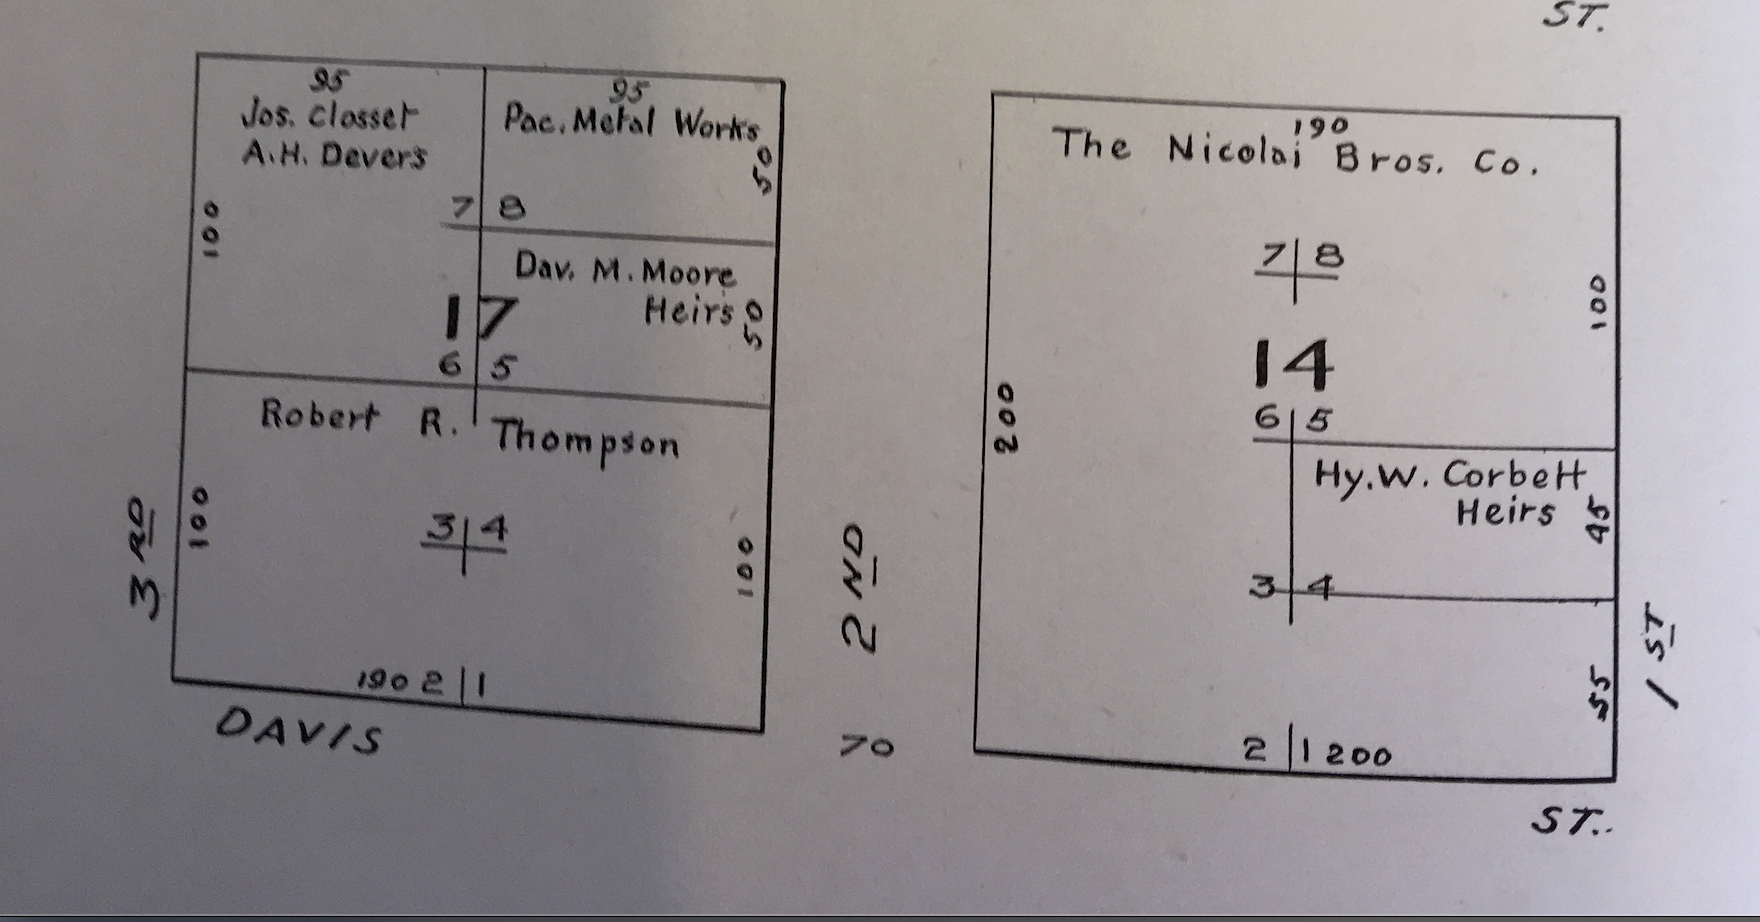
\includegraphics{images/image19.png}
\caption{alt\_text}
\end{figure}

Sedelia Stafford-Hohmann-Price-Thode died August 30, 1961, at 2723 N
Halleck, still living with Irene (now Irene Pettis).

.

{\textgreater\textgreater\textgreater\textgreater\textgreater{}
gd2md-html alert: inline image link here (to images/image20.png). Store
image on your image server and adjust path/filename/extension if
necessary. }(Back to top)(Next
alert){\textgreater\textgreater\textgreater\textgreater\textgreater{} }

\begin{figure}
\centering
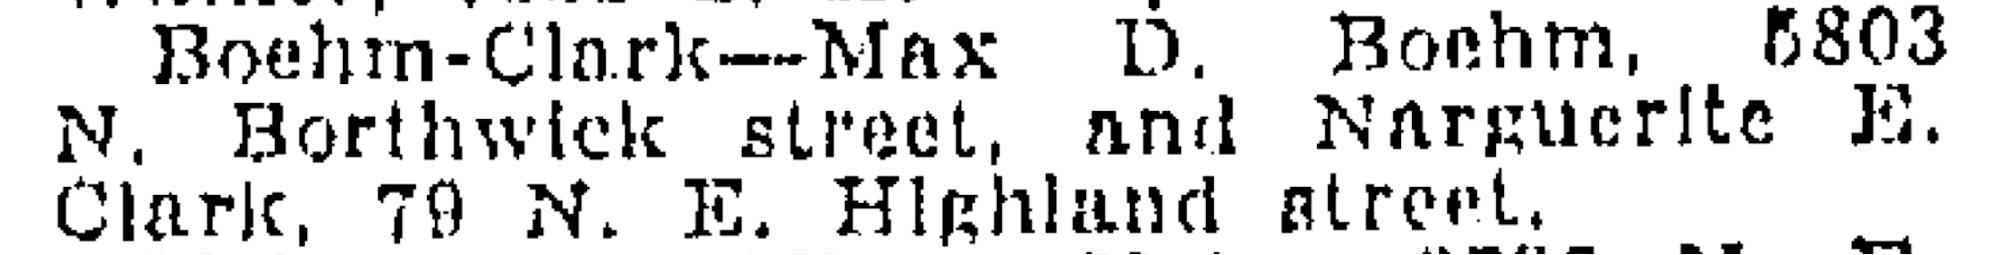
\includegraphics{images/image20.png}
\caption{alt\_text}
\end{figure}

\hypertarget{section-4}{%
\subsection{}\label{section-4}}

\hypertarget{ericksons-and-grahams}{%
\subsection{Ericksons and Grahams}\label{ericksons-and-grahams}}

We have followed Delia all the way until she left this earthly coil, but
there is still more to tell about the lot and the house at what is now
107 NE Bryant Street.

On September 13, 1930 ``\emph{Sidelia F. Thode, a widow, also known as
S. F. Thode}'', sold the house for ``\emph{ten (10) dollars and other
valuable considerations}'' to Hjalmar J. Erickson and Irene M. Erickson,
husband and wife. The deed says

\begin{verbatim}
_… that the above granted premises are free from all incumbrances except mortgage indebtedness as of record, city liens and taxes, all of which the grantees herein named assume and agree to pay …_


_[https://drive.google.com/open?id=1yfD0fdhuGeJOsEu2g896K2Nwvh2DNy2B](https://drive.google.com/open?id=1yfD0fdhuGeJOsEu2g896K2Nwvh2DNy2B)_
\end{verbatim}

Then on July 3, 1935 the North American Life Insurance Company of
Chicago sues ``\emph{Hjalmar J. Erickson and Irene M. Erickson, Husband
and Wife; Merkle Investment Company, and Oregon Corporation; and William
L. Graham}'' in Multnomah Circuit Court for the foreclosure of a
mortgage. The judge in suit number 118384 issues an Execution and Order
of Sale for the property, and as a consequence there is a sheriff's sale
on August 5, 1935. The highest bidder at the public auction at the
courthouse door is the North American Life Insurance Company, and they
take possession for the sum of \$ 3038.57, which could be the amount due
on the mortgage.

\url{https://drive.google.com/open?id=1z8gjP-YCEQnwiIrA4V2ZdV-tu0C2evUe}

On November 19, 1935 Hjalmar J. Erickson and Irene M. Erickson deeded
their remaining interest in the property to the North American Life
Insurance Company of Chicago, Illinois, for ``one and no/100 dollars (\$
1.00) and other good and valuable considerations''. The deed stipulated:

\begin{verbatim}
_The intention of this conveyance is to forever bar all the right, title and interest of the above named grantors in and to the above described real property, including their statutory right of redemption from sheriff’s sale in that suit No. 118384, in the Circuit Court of the State of Oregon for Multnomah County._


_[https://drive.google.com/open?id=14OHJqXHAEaioPdbwxqdUXyRLX0DBErPf](https://drive.google.com/open?id=14OHJqXHAEaioPdbwxqdUXyRLX0DBErPf)_
\end{verbatim}

There is also a quitclaim on that same November 19, 1935 in which
William L. Graham and Eva L. Graham sell their rights to the property
for \$ 1.00 to the same Life Insurance company.

\url{https://drive.google.com/open?id=17rrRgoEs_-fn0g5_DvGbQkQRVPgBxDBe}

\hypertarget{harry-a.-montag}{%
\subsection{Harry A. Montag}\label{harry-a.-montag}}

And then, on February 19, 1938, Harry A. and Esther Montag bought lots 7
to 9 in block 19 of Love's Addition, and of course the house on it, from
the North American Life Insurance Company Inc.~for the nominal sum of
ten dollars. Here is a clip of the relevant index file from the
Multnomah County Records Office.

{\textgreater\textgreater\textgreater\textgreater\textgreater{}
gd2md-html alert: inline image link here (to images/image21.png). Store
image on your image server and adjust path/filename/extension if
necessary. }(Back to top)(Next
alert){\textgreater\textgreater\textgreater\textgreater\textgreater{} }

\begin{figure}
\centering
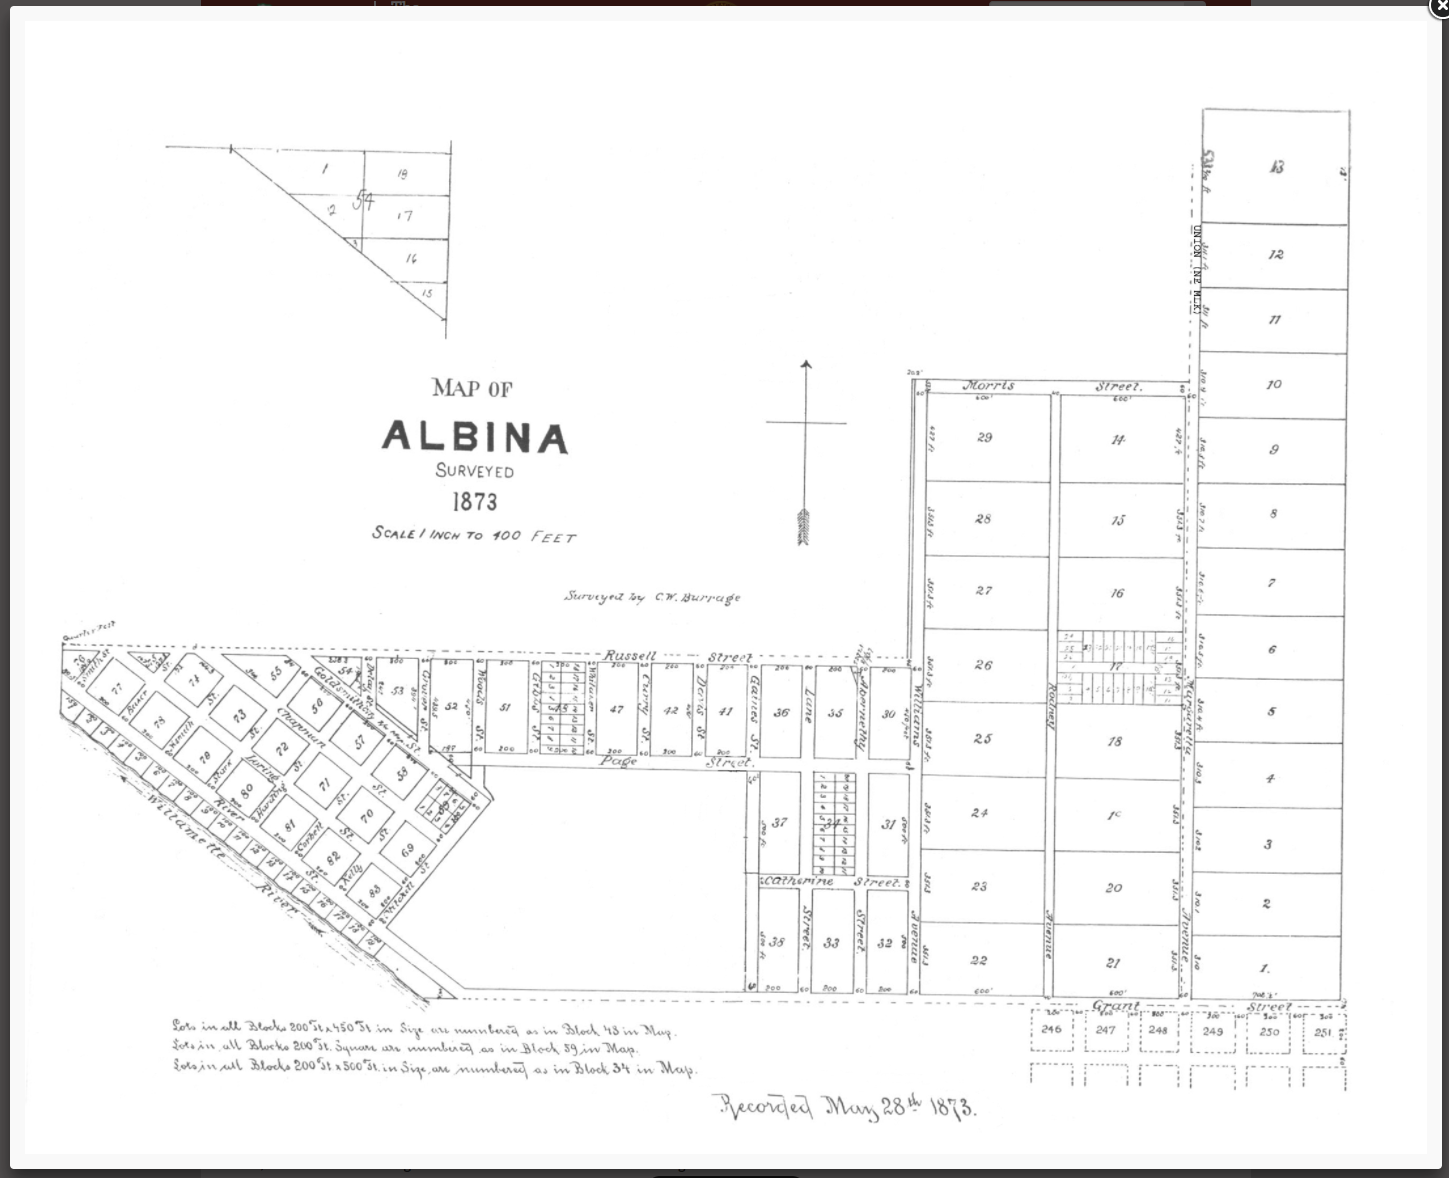
\includegraphics{images/image21.png}
\caption{alt\_text}
\end{figure}

The deed specifies that \emph{``the above granted premises are free from
all encumbrances, except taxes payable during the year 1938 and balance
due on city lien dated July 11, 1928.''}

\emph{\url{https://drive.google.com/open?id=1wf-1nSkWrHVHBtovCNtE-d6XMuk0zDNe}}

Somebody, not me, could easily write a book about the history of the
Montag family and the Montag business in Portland. For our purposes it
suffices to briefly review some of the main facts. The company, known as
the Portland Stove Works or the Montag Stove and Furnace Works, was
established in 1883 by John Montag on Hood Street. They manufactured
more than 300 models of kitchen and heating stoves, and in addition
provided parts and repairs for other makes. In addition John Montag was
a force in the Democratic Party of Oregon, he served on the executive
board as chairman of the Fire Commission for mayors Lane and Pennoyer,
and eventually he became a member of the City Council for the sixth
ward.

The Montag firm was family owned and operated until 1955, when it
incorporated. There is an article in the Orgonian of January 25, 1955
that shows that the stove works provided gainful employment to many, if
not most, male members of the Montag family.

{\textgreater\textgreater\textgreater\textgreater\textgreater{}
gd2md-html alert: inline image link here (to images/image22.png). Store
image on your image server and adjust path/filename/extension if
necessary. }(Back to top)(Next
alert){\textgreater\textgreater\textgreater\textgreater\textgreater{} }

\begin{figure}
\centering
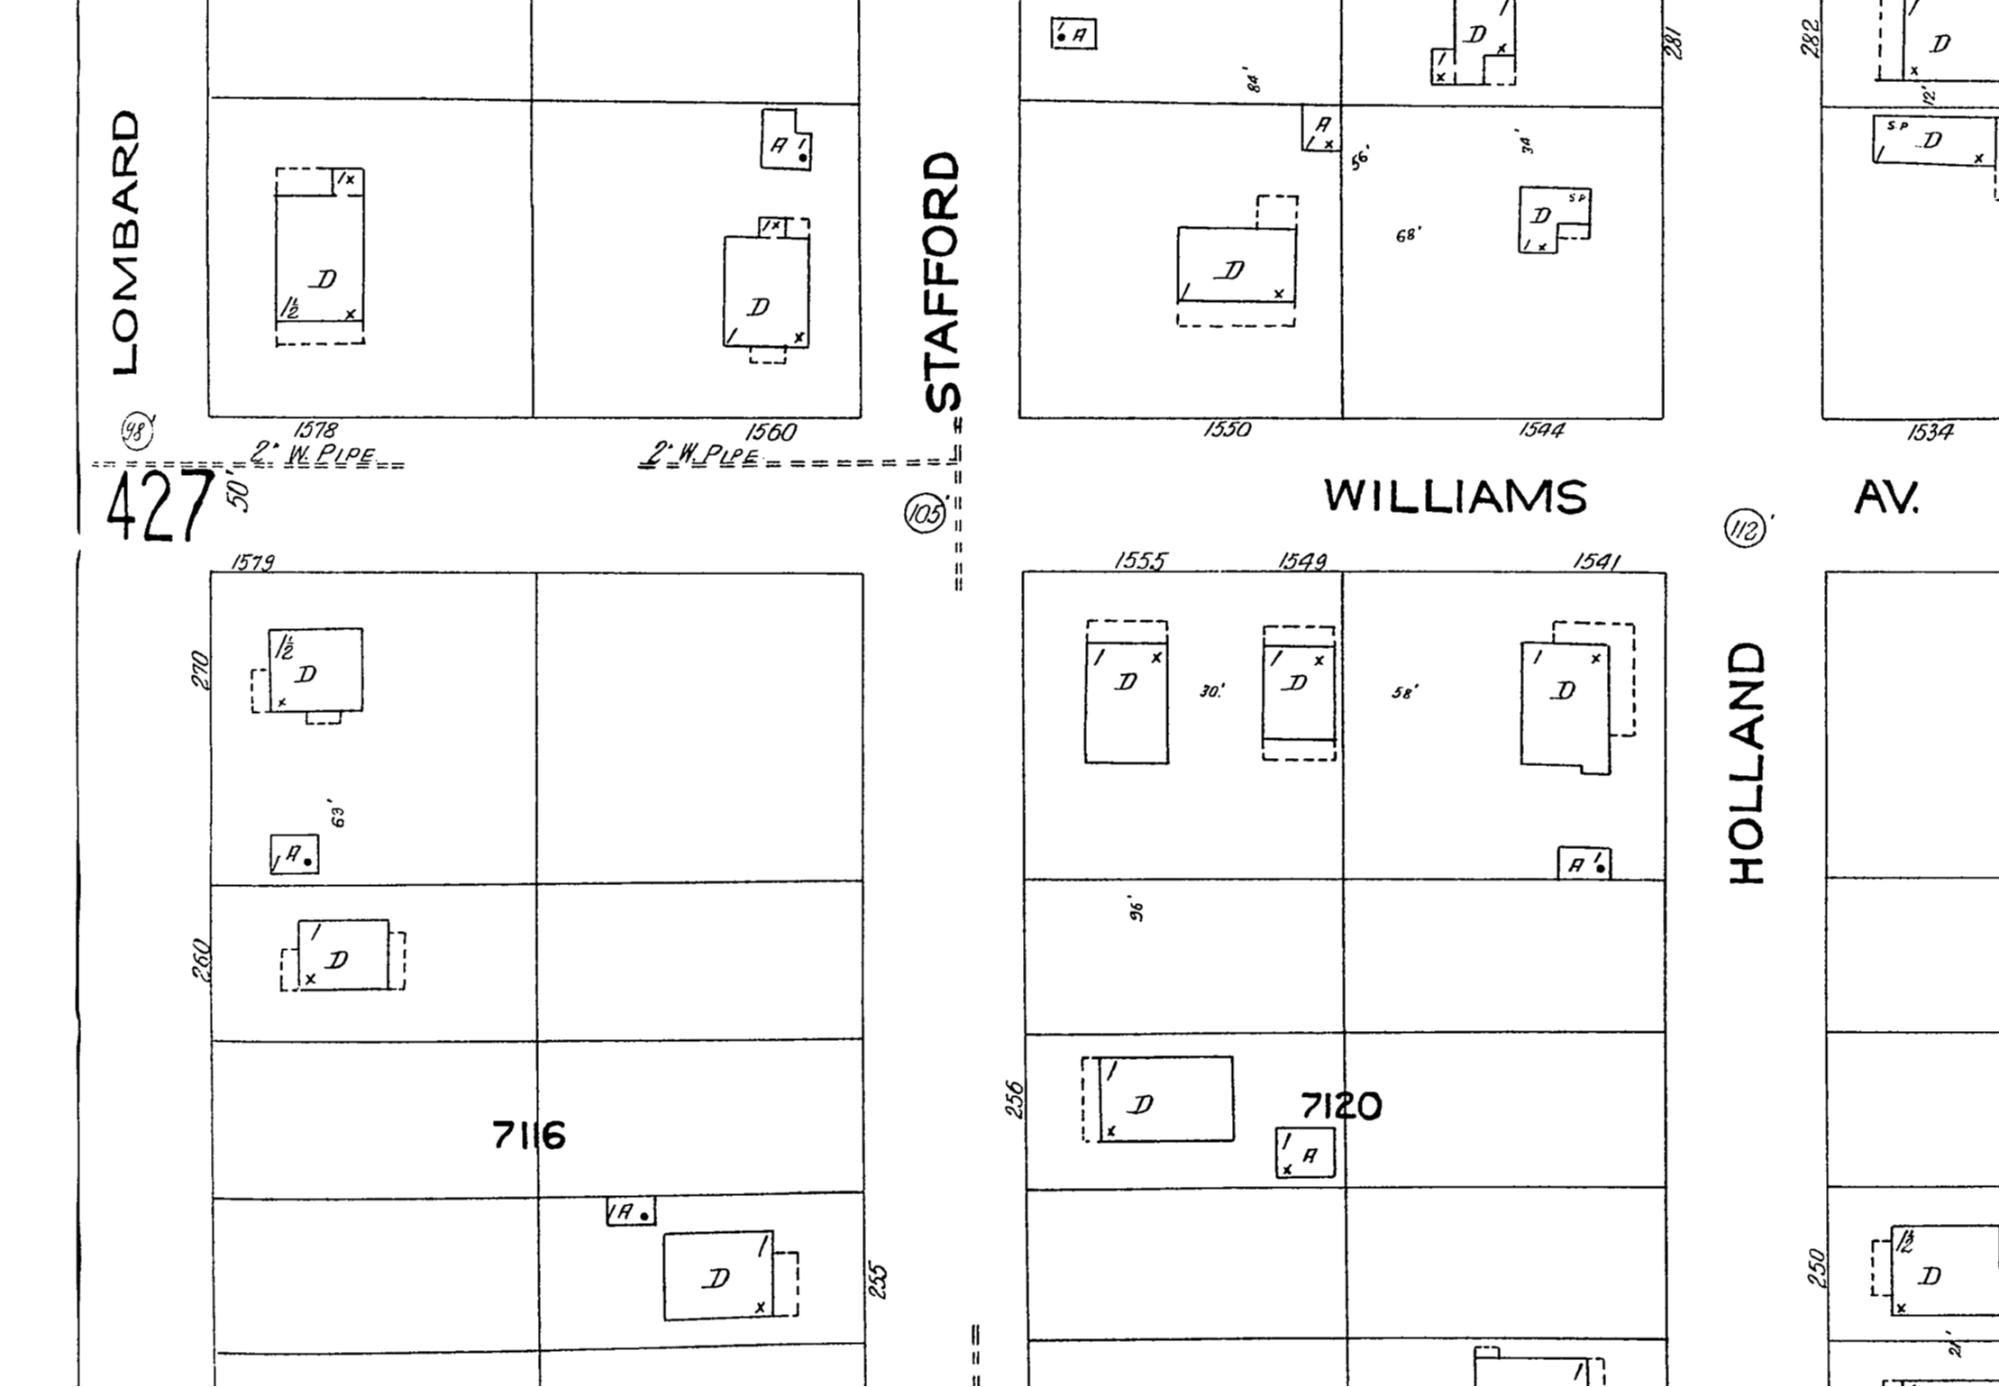
\includegraphics{images/image22.png}
\caption{alt\_text}
\end{figure}

Harry Albert Montag was born in 1896, son of William and Sophia Montag.
William (originally Wilhelm) arrived in the US in 1858, married Sophia
Petrie in Illinois in 1880, and moved to Portland to join the Montag
family business. As an aside, if we go through the census records we see
that in both 1910 and 1930 the Montags gave their name as Montague.

Harry lived at home, at 803 Commercial Street, until at least 1927. He
married Esther Olsen in 1924. In the 1930 census their address is 92
Bryant Street, which became 1008 North Bryant Street after the Great
Renumbering. We know he sold this home in 1938, and that he had arrived
at 107 Northeast Bryant in 1940, accompanied by Esther and his three
children Helen, Richard, and Daniel. The Oregonian of September 18, 1938
has a picture of the fairly unassuming house they moved out of.

{\textgreater\textgreater\textgreater\textgreater\textgreater{}
gd2md-html alert: inline image link here (to images/image23.png). Store
image on your image server and adjust path/filename/extension if
necessary. }(Back to top)(Next
alert){\textgreater\textgreater\textgreater\textgreater\textgreater{} }

\begin{figure}
\centering
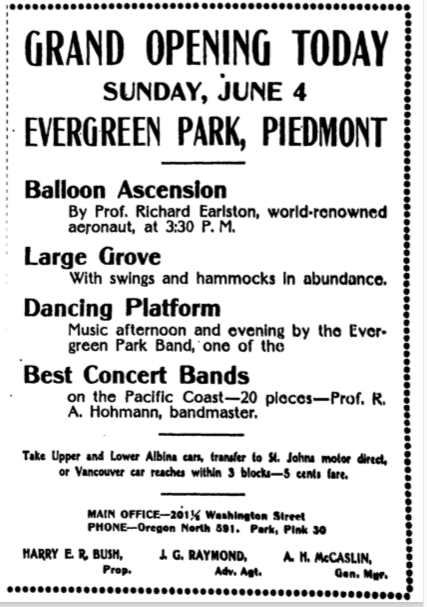
\includegraphics{images/image23.png}
\caption{alt\_text}
\end{figure}

The most recent edition of the Sanborn maps is updated until about 1950.

{\textgreater\textgreater\textgreater\textgreater\textgreater{}
gd2md-html alert: inline image link here (to images/image24.png). Store
image on your image server and adjust path/filename/extension if
necessary. }(Back to top)(Next
alert){\textgreater\textgreater\textgreater\textgreater\textgreater{} }

\begin{figure}
\centering
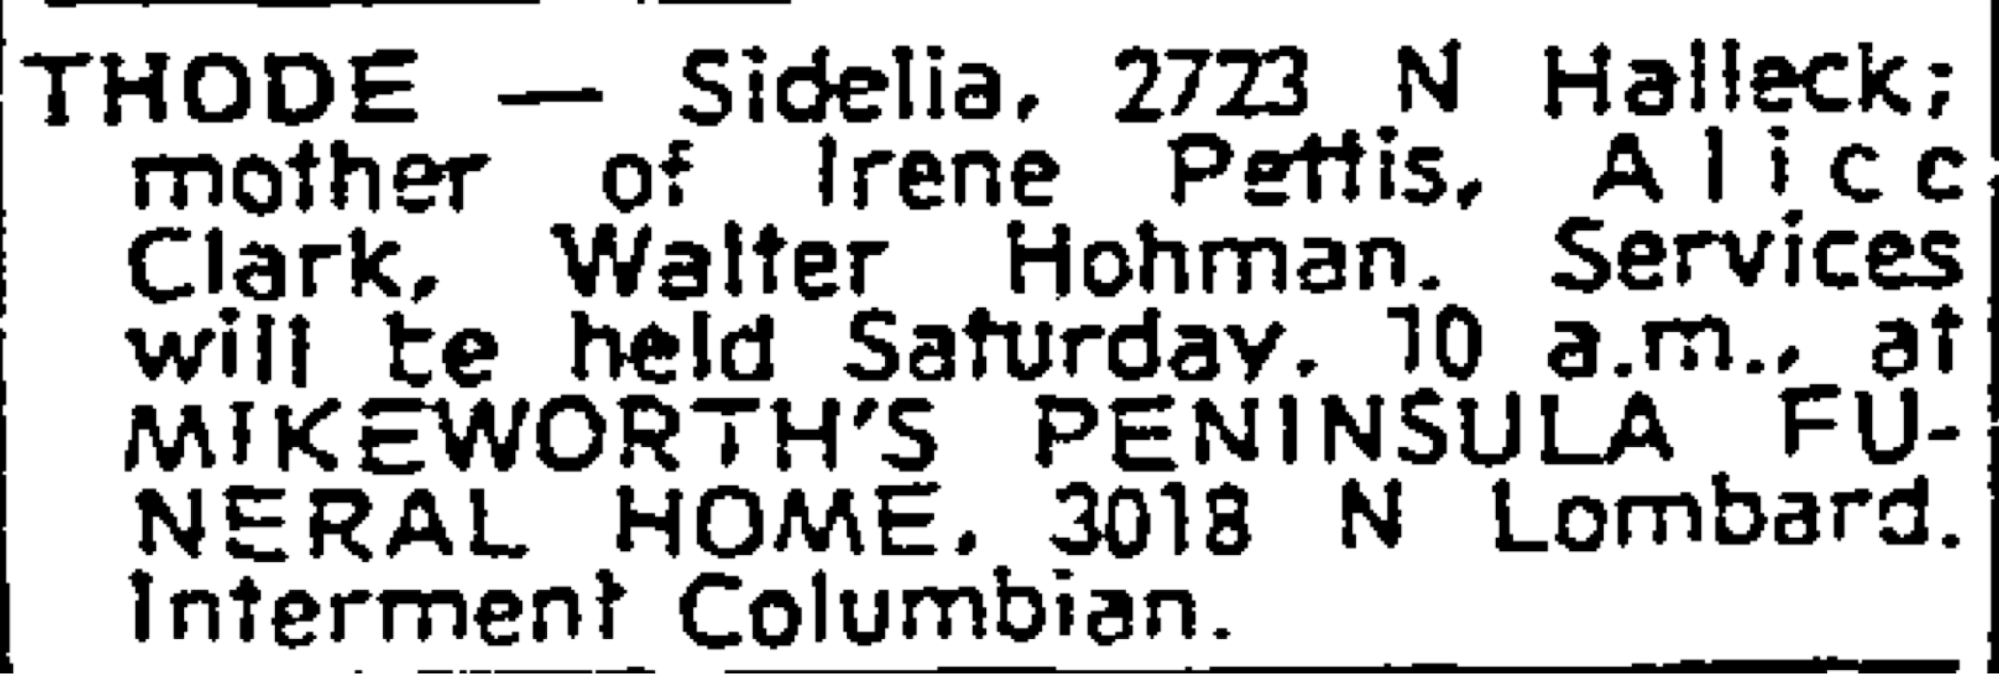
\includegraphics{images/image24.png}
\caption{alt\_text}
\end{figure}

City directories tell us that the Montags still lived at 107 Northeast
Bryant in 1955, but after that the information in the paper and the
records on ancestry.com become scarce. Harry lived until 1977 and Esther
until 1996, but I am not sure yet where they spent their remaining days,
and when 107 Northeast Bryant was sold to the next owner. I will look
for the relevant deeds, of course, but for now I'll stop here.

\end{document}
